%% 
%% Copyright 2019-2024 Elsevier Ltd
%% 
%% This file is part of the 'CAS Bundle'.
%% --------------------------------------
%% 
%% It may be distributed under the conditions of the LaTeX Project Public
%% License, either version 1.3c of this license or (at your option) any
%% later version.  The latest version of this license is in
%%    http://www.latex-project.org/lppl.txt
%% and version 1.3c or later is part of all distributions of LaTeX
%% version 1999/12/01 or later.
%% 
%% The list of all files belonging to the 'CAS Bundle' is
%% given in the file `manifest.txt'.
%% 
%% Template article for cas-sc documentclass for 
%% double column output.

\documentclass[a4paper,fleqn]{cas-sc}

% If the frontmatter runs over more than one page
% use the longmktitle option.

%\documentclass[a4paper,fleqn,longmktitle]{cas-sc}

%\usepackage[numbers]{natbib}
%\usepackage[authoryear]{natbib}
\usepackage[authoryear,longnamesfirst]{natbib}

\usepackage{algorithm}
\usepackage[noend]{algorithmic}
\usepackage{subcaption} 
\usepackage{enumitem}

%%%Author macros
\usepackage{amssymb}
\usepackage{xspace}

\newcommand{\even}          {\raisebox{0.0ex}{\scalebox{1.0}{$\bigcirc$}}\xspace}
\newcommand{\odd}           {\scalebox{0.9}{$\square$}\xspace}
\newcommand{\subeven}       {\raisebox{0.3ex}{\scalebox{0.7}{$\bigcirc$}}\xspace}
\newcommand{\subodd}        {\scalebox{0.6}{$\square$}\xspace}
\newcommand{\player}        {\mathsf{p}\xspace}
\newcommand{\opponent}      {\overline{\mathsf{p}}\xspace}

\newcommand{\wregularform}  {$\omega$-regular form\xspace}
\newcommand{\wregulargame}  {$\omega$-regular game\xspace}
\newcommand{\wregulargames} {$\omega$-regular games\xspace}
\newcommand{\noc}           {{\textsf{NOC}}\xspace}
\newcommand{\nooppc}        {{\small\textsf{No\textit{-}Opponent\textit{-}Cycle}}\xspace}
\newcommand{\nocchecker}    {{\small\textsf{NOC\textit{-}Checker}}\xspace}
\newcommand{\noceager}      {{\small\textsf{NOC\textit{-}Eager}}\xspace}
\newcommand{\nocfilter}     {{\small\textsf{NOC\textit{-}Filter}}\xspace}
\newcommand{\nocmemo}       {{\small\textsf{NOC\textit{-}Memo}}\xspace}
\newcommand{\nocbrancher}   {{\small\textsf{NOC\textit{-}Brancher}}\xspace}
\newcommand{\nocq}          {{\small\textsf{NOCQ}}\xspace}
\newcommand{\zra}           {{\small\textsf{ZRA}}\xspace}
\newcommand{\closerdots}    {.\kern-0.05em.\kern-0.05em.}
\newcommand{\todo}[1]       {\textcolor{red}{To Do: #1}}

\newtheorem{definition}{Definition}
\newtheorem{example}{Example}

% % Define MiniZinc syntax highlighting
% \lstdefinelanguage{MiniZinc}{
%   keywords={include, constraint, output, array, of, var, bool},
%   morekeywords={[2] set, int, float, string},
%   keywordstyle=\color{blue}\bfseries,
%   keywordstyle={[2]\color{teal}\bfseries},
%   sensitive=true,
%   comment=[l]{\%}, 
%   morecomment=[s]{/*}{*/},
%   commentstyle=\color{gray}\ttfamily,
%   stringstyle=\color{red}\ttfamily,
%   morestring=[b]",    % Defines double-quoted strings
%   morestring=[b]',    % Defines single-quoted strings  basicstyle=\ttfamily\small,
%   numberstyle=\tiny\color{gray},
%   numbers=left,
%   stepnumber=1,
%   breaklines=true,
%   showstringspaces=false,
%   frame=single,
%   tabsize=2,
%   basicstyle=\ttfamily\footnotesize
% }

% \lstset{
%     basicstyle=\small\ttfamily,
%     backgroundcolor=\color{gray!10},
%     frame=single,
%     framerule=0pt,
%     columns=fullflexible,
%     breaklines=true,
%     xleftmargin=0.5em,
%     xrightmargin=0.5em
% }


\def\tsc#1{\csdef{#1}{\textsc{\lowercase{#1}}\xspace}}
\tsc{WGM}
\tsc{QE}
%%%

% Uncomment and use as if needed
%\newtheorem{theorem}{Theorem}
%\newtheorem{lemma}[theorem]{Lemma}
%\newdefinition{rmk}{Remark}
%\newproof{pf}{Proof}
%\newproof{pot}{Proof of Theorem \ref{thm}}

\begin{document}
\let\WriteBookmarks\relax
\def\floatpagepagefraction{1}
\def\textpagefraction{.001}

% Short title
\shorttitle{Constraint Parity Games}


% Main title of the paper
\title [mode = title]{A Constraint-based Approach for Solving Parity Games}  

% Title footnote mark
% eg: \tnotemark[1]
% \tnotemark[1] 

% Title footnote 1.
% eg: \tnotetext[1]{Title footnote text}
% \tnotetext[1]{} 

% First author
%
% Options: Use if required
% eg: \author[1,3]{Author Name}[type=editor,
%       style=chinese,
%       auid=000,
%       bioid=1,
%       prefix=Sir,
%       orcid=0000-0000-0000-0000,
%       facebook=<facebook id>,
%       twitter=<twitter id>,
%       linkedin=<linkedin id>,
%       gplus=<gplus id>]
% Short author running head (up top with \shorttitle)
\shortauthors{G. Hernandez et al.}

% First Author (Dual affiliation [1,2], Corresponding Author)
\author[1,2]{Gonzalo Hernandez}[orcid=0000-0002-9740-2625]
\cormark[1]
\ead{gonzalo.hernandez@udenar.edu.co}
\credit{Conceptualization, Methodology, Software, Writing - original draft}

% Second Author
\author[1]{Julian Garcia}
\ead{Julian.Garcia@monash.edu}
\credit{Writing - review \& editing}

% Third Author
\author[3]{Julian Gutierrez}
\ead{J.Gutierrez@sussex.ac.uk}
\credit{Writing - review \& editing}

% Fourth Author
\author[1]{Jip Dekker}
\ead{Jip.Dekker@monash.edu}
\credit{Software, Writing - review \& editing}

% Fifth Author
\author[1]{Guido Tack}
\ead{guido.tack@monash.edu}
\credit{Supervision, Methodology, Writing - review \& editing}


\affiliation[1]{organization={Faculty of Information Technology, Monash University},
            state={Victoria},
            country={Australia}}

\affiliation[2]{organization={Departamento de Sistemas, Universidad de Nariño},
            state={Nariño},
            country={Colombia}}

\affiliation[3]{organization={Department of Informatics, University of Sussex},
            state={Brighton},
            country={United Kingdom}}


\cortext[1]{Corresponding author}

% Footnote text
% \fntext[1]{}

% For a title note without a number/mark
%\nonumnote{}

% \newpage
% \tableofcontents
% \newpage

% Here goes the abstract
\begin{abstract}
Solving parity games is a central task in formal verification, particularly within model checking and synthesis methods that see widespread industrial application. In this paper, we introduce a constraint-based method for parity games powered by a novel propagation algorithm that eliminates opponent cycles from the game graph. This technique produces an efficient solver by capitalizing on the inherent duality between both players. Implemented within a Lazy Clause Generation framework, our approach surpasses all existing constraint-based solvers and competes closely with state-of-the-art specialized non-CP algorithms—frequently matching or exceeding their performance—while preserving the adaptability of general constraint systems.

Because extra constraints can be seamlessly integrated, our framework provides a flexible way to refine problem models and target preferred solutions under supplementary conditions. This adaptability also enables the resolution of parity games bound by additional quantitative constraints, such as cost or resource limits. We present the theoretical foundation of this approach, an empirical evaluation, and an analysis of the results, including a performance comparison across different variants of the new propagator.
\end{abstract}

% Use if graphical abstract is present
%\begin{graphicalabstract}
%\includegraphics{}
%\end{graphicalabstract}

% Research highlights
% \begin{highlights}
% \item 
% \item 
% \item 
% \end{highlights}


% Keywords
% Each keyword is seperated by \sep
\begin{keywords}
Constraint programming  \sep Parity games \sep Verification.
\end{keywords}

\maketitle

% \newpage
\section{Introduction}
%Parity games are two-player zero-sum infinite-duration games played on a labeled directed graph, where vertices represent states of the players in the game and edges represent their possible available actions at every state. Solving these games is central to several techniques in automated formal verification, in particular for solving model checking and automated synthesis problems.

%Since parity games are zero-sum, perfect-information games, solving them amounts to finding which player (usually called Player Even, or $\even$, and Player Odd, or $\odd$) has a winning strategy from a given starting vertex in the graph. It is known that deciding the winner in parity games is an $\mathsf{NP} \cap \mathsf{co\textit{-}NP}$ problem~\citep{Jurdziński:1998}, but it is not known whether or not they can be solved in polynomial time; a problem that has remained open for nearly 50 years. 
% Due to the importance of parity games in formal verification, several algorithms have been developed \citep{Aggarwal:2023,Benerecetti:2025,Jurdziński:2000,Jurdziński:2022,Zielonka:1998}, all of which suffer from exponential running time limitations for specific classes of games. One such approach involves reducing the solution of a parity game to the solution of a SAT instance representing the game. The generated SAT instance is satisfiable if and only if Player Even has a winning strategy in the original game. This idea has a lot of potential given the advances in SAT-solving technology, but, as we will show later, it suffers from poor scalability due to the large size of the generated CNF formula for a given game.

%In this paper, we address these scalability issues by developing a specialised propagator that takes into account the structure of parity games, resulting in significant improvements in performance and modelling power. In particular, we show that our method outperforms all other state-of-the-art constraint-based solvers.
% Specifically, we propose replacing the SAT-based encoding used to forbid cycles corresponding to Player Odd wins in the game graph \citep{Heljanko:2012} with a set of efficient global constraint propagators; this significantly reduces the encoding size of the problem. Two of the proposed propagators are based on depth-first search, and a third is a checker that analyses the strongly connected components (SCCs) of the game graph. These propagators filter edges that would close winning cycles for a selected opponent player and generate explanations for each filtering step, enabling their integration into a Lazy Clause Generation solver~\citep{DBLP:journals/constraints/OhrimenkoSC09}.

%We show that our implementation not only outperforms existing SAT and CP-based approaches but also achieves performance comparable to that of state-of-the-art specialized non-CP-based algorithms, often matching or exceeding their results. This work contributes to establishing the CP framework as a practical tool for solving both general and specialized classes of parity games.

%The remainder of this paper is organized as follows. We first present the theoretical foundations and necessary definitions used in further sections, and then introduce our proposed approach -- including the design and implementation of the \noc propagators. After that, we provide different experimental results, a comparative analysis against state-of-the-art solvers, and present the extension of our method with additional constraints. At the end of the paper, we focus on the presentation of a number of concluding remarks, a discussion of our main findings, and some proposals for potential future research directions.


Parity games are two-player zero-sum infinite-duration games played on a labeled directed graph, where vertices represent states of the players in the game and edges represent their possible available actions at every state. 
Solving these games is central to several techniques in automated formal verification, in particular for solving model checking and automated synthesis problems.
%
More broadly, parity games provide a canonical algorithmic representation of
$\omega$-regular winning conditions and arise naturally in the analysis of
systems whose specifications involve nested least and greatest fixpoints.
In particular, solving parity games is closely connected to model checking
for the modal $\mu$-calculus, automata-theoretic verification, and the
synthesis of reactive systems~\citep{vanDijk:2018,Zielonka:1998,Luttenberger:2020}.
This connection is especially useful because parity games admit
\emph{memoryless} winning strategies: whenever a player can win from a
vertex, it can do so using a strategy that depends only on the current
vertex. Consequently, algorithms for parity games can serve both as decision
procedures and as mechanisms for extracting finite witnesses that can be
interpreted as strategies or controllers.

Since parity games are zero-sum, perfect-information games, solving them amounts to finding which player (usually called Player Even, or $\even$, and Player Odd, or $\odd$) has a winning strategy from a given starting vertex in the graph. 
It is known that deciding the winner in parity games belongs to
$\mathsf{UP} \cap \mathsf{co\text{-}UP}$, and therefore also to
$\mathsf{NP} \cap \mathsf{co\text{-}NP}$~\citep{Jurdziński:1998}, but it
remains unknown whether parity games can be solved in polynomial time.
%
The complexity landscape nevertheless changed substantially with the
development of the first quasi-polynomial-time algorithms for parity
games~\citep{Calude:2017,JurdzinskiLazic:2017}. Several subsequent approaches
have obtained quasi-polynomial bounds through different characterisations of
the problem~\citep{Parys:2019,Jurdziński:2022}. At the same time, specialised
algorithms such as progress measures, recursive algorithms, and priority
promotion remain highly effective in practice~\citep{Jurdziński:2000,
Benerecetti:2025,vanDijk:2018}. Thus, parity games present an interesting
algorithmic situation: their precise polynomial-time complexity is unresolved,
strong worst-case algorithms are known, and highly optimised specialised
methods perform very well empirically. This makes them an informative
case to determine if more general solving frameworks can achieve
comparable performance while retaining greater modelling flexibility.

A different approach consists of reducing the solution of a parity game to
a constraint problem, for example to a SAT instance representing the game.
The generated SAT instance is satisfiable if and only if Player Even has a
winning strategy in the original game. 
This idea has a lot of potential given the advances in SAT-solving technology,
but, as we will show later, it suffers from poor scalability due to the large
size of the generated CNF formula for a given game.

This limitation raises a more general question in constraint processing and
automated reasoning: how much of the structure of a problem should be exposed
directly to the solver rather than compiled into a generic low-level
representation? The parity condition provides a particularly clear instance
of this question. It is inherently a global property of an infinite play:
whether a play is winning depends on the priorities that recur indefinitely,
rather than on any individual transition considered in isolation.
Encoding such a property using large collections of low-level variables
and constraints can obscure the graph structure from which the condition
originates. Constraint Programming (CP), in contrast, allows domain-specific
reasoning to be encapsulated within \emph{global constraints}, while
specialised propagators can exploit the underlying combinatorial structure
directly~\citep{Apt:2003,Rossi:2006}. When combined with Lazy Clause Generation
(LCG), such propagators can additionally explain their inferences as clauses,
combining problem-specific propagation with the conflict learning mechanisms
that make modern SAT solving so incredibly effective in practice~\citep{DBLP:journals/constraints/OhrimenkoSC09,
Stuckey:2010}.

In this paper, we address these scalability issues by developing a specialised propagator that takes into account the structure of parity games, resulting in significant improvements in performance and modelling power. 
In particular, we show that our method {\em outperforms all other state-of-the-art constraint-based solvers} in the literature. 

The key observation underlying our approach is that, once the choices of a
positional strategy are represented in the game graph, the parity condition
can be characterised through its recurrent cycle structure. Since the arena
is finite, every infinite play eventually revisits vertices, and the winner
is determined by the highest priority occurring in the recurrent part of the
play. From the perspective of one player, it is therefore sufficient to rule
out reachable cycles whose highest priority favours the opponent. This gives
a direct graph-theoretic interpretation of the winning condition and motivates
our \emph{No-Opponent-Cycle} (\noc) constraint: rather than representing the
parity condition indirectly through a large auxiliary encoding, the solver
reasons directly about the cycles that would invalidate a candidate winning
strategy.

Specifically, we propose replacing the SAT-based encoding used to forbid cycles corresponding to Player Odd wins in the game graph~\citep{Heljanko:2012} with a set of efficient global constraint propagators; this significantly reduces the encoding size of the problem. Two of the proposed propagators are based on depth-first search, and a third is a checker that analyses the strongly connected components (SCCs) of the game graph. These propagators filter edges that would close winning cycles for a selected opponent player and generate explanations for each filtering step, enabling their integration into a Lazy Clause Generation solver~\citep{DBLP:journals/constraints/OhrimenkoSC09}.

An additional feature of this formulation is that it treats the two players
symmetrically. Because parity games are determined, proving that one player
cannot satisfy its winning constraints establishes that the other player
wins. The cost of finding a winning strategy and the cost of refuting one
need not be symmetric on a particular instance. We therefore exploit this
duality by solving the game from both players' perspectives, allowing the
computation to terminate as soon as either search establishes the winner.
As our experiments show, this is particularly effective in conjunction with
LCG, where many instances are resolved through comparatively short
unsatisfiability proofs.

We show that our implementation not only outperforms existing SAT and CP-based approaches but also achieves performance comparable to that of state-of-the-art specialized non-CP-based algorithms, often matching or exceeding their results. This work contributes to establishing the CP framework as a practical tool for solving both general and specialized classes of parity games, as well as some extensions with quantitative features. 

Indeed, the use of a general constraint framework also provides a second advantage
that is largely orthogonal to raw solving performance. In verification and
synthesis applications, one may be interested not only in whether a winning
strategy exists, but in strategies satisfying additional structural or
quantitative requirements. Examples include resource or energy constraints,
cost bounds, or restrictions on the strategies that may be selected
\citep{ChatterjeeD12,Fijalkow:2014,Weinert:2016}. Such requirements typically
require modifications to specialised game-solving algorithms. In a CP model,
by contrast, they can be expressed as additional constraints while retaining
the same core parity-game propagator. We use this flexibility later in the
paper to illustrate how the framework can be adapted to constrained synthesis
and quantitative variants of parity games.

More generally, the approach explored in this paper illustrates a broader
methodology for symbolic AI and automated reasoning. Many combinatorial
reasoning problems admit highly specialised algorithms that exploit their
mathematical structure, while general-purpose declarative solvers offer
greater modelling flexibility but may lose some of this structure when the
problem is compiled into low-level constraints. Global constraints provide
a way of bridging these two approaches: problem-specific reasoning can be
encapsulated in specialised propagators while search, learning, and the
interaction with additional constraints remain delegated to a general-purpose
solver. Parity games provide a particularly demanding setting in which to
study this trade-off, since highly optimised specialised algorithms are
available and the winning condition has a rich global graph structure. Our
results therefore investigate not only a new way of solving parity games in practice,
but also the extent to which domain-specific symbolic reasoning can be
integrated effectively within a general constraint-solving architecture.

This article substantially extends our preliminary conference
work~\citep{Hernandez:2026:noc}. In addition to a more detailed presentation
of the \noc framework and its propagators, we investigate alternative
constraint formulations and solver back ends, compare against CP and SMT
encodings of the progress measure, provide an expanded analysis
of search strategies and the duality between the two players, study resource
utilisation and scalability on larger instances, and examine how the same
constraint-based framework can accommodate additional requirements on
winning strategies.

The remainder of this paper is organized as follows. We first present the theoretical foundations and necessary definitions used in further sections, and then introduce our proposed approach -- including the design and implementation of the \noc propagators. After that, we provide different experimental results, a comparative analysis against state-of-the-art solvers, and present the extension of our method with additional constraints. At the end of the paper, we focus on the presentation of a number of concluding remarks, a discussion of the main findings, and some proposals for potential future research directions.

\section{Preliminaries and Related Work}

This section introduces parity games and overviews the existing translations into Boolean Satisfiability (SAT) and Satisfiability Modulo Theories (SMT).

\subsection{Parity Games}

Parity games are two-player zero-sum games played on a labeled directed graph, called the \textit{arena}, where two players, \textit{Even} and \textit{Odd} (denoted~\even or 0, and~\odd or 1, respectively), move a token along adjacent vertices depending on which player controls the current vertex. This process generates a path of states visited by the token. In a parity game, each path is winning for either Player \even or Player \odd. The goal of each player is to enforce a winning path in their favour. We now formalize parity games, including the definition of when a given path in the graph is winning for either player.

\subsubsection{Arenas, Strategies, and Plays.}

A game arena is a tuple $\mathcal{A} = (V_{\subeven}, V_{\subodd}, E, \Omega)$, where $V = V_{\subeven} \cup V_{\subodd}$ is a finite set of vertices, partitioned into \( V_{\subeven} \) (controlled by Player~\even) and \( V_{\subodd} \) (controlled by Player~\odd),
%
$E \subseteq V \times V$ is a set of directed edges where every vertex has at least one successor,
%
and $\Omega: V \to \mathbb{N}$ is a labeling function that assigns to each vertex a non-negative integer, called its \textit{priority}.
%
For any vertex \( v \in V \), we write \( vE = \{ w \in V \mid (v, w) \in E \} \) for its set of successors (adjacent to outgoing edges from \( v \)), and \( Ev = \{ u \in V \mid (u, v) \in E \} \) for its set of predecessors (adjacent to incoming edges to \( v \)).

The game starts with a token at an initial vertex $v_0 \in V$. Player Even is responsible for moving the token when it is on a vertex in $V_{\subeven}$, and Player Odd is responsible for moving the token when it is on a vertex in $V_{\subodd}$. Because every node is required to have at least one outgoing edge, the token travels along the graph generating a path of infinite length. The winner is determined by the highest priority that is visited by the token infinitely often. Figure~\ref{fig:game01} illustrates an instance of a parity game arena.

\begin{figure}
    \centering
    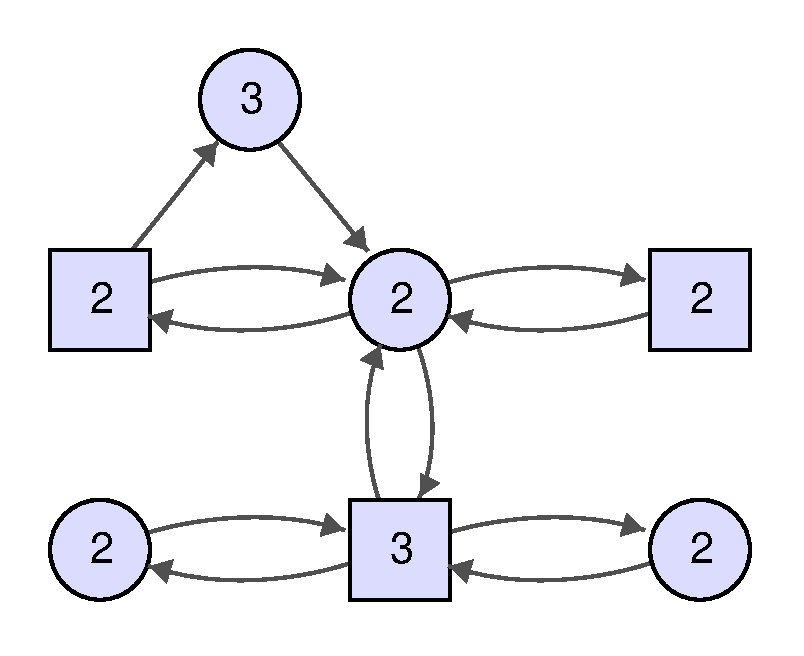
\includegraphics[width=0.35\textwidth]{images/game01} 
    \caption{A parity game with 7 vertices and 12 edges. Each vertex carries a priority from the set $\{2,3\}$. Vertices controlled by Player~$\even$ are shown as circles, while vertices controlled by Player~$\odd$ are shown as squares.}
    \label{fig:game01}
\end{figure}

\subsection*{Strategies, Plays, and Winning Conditions}
A memoryless or {\em positional strategy} for player Even (player Odd) is a function $f_{\subeven} : V_{\subeven} \to V$ ($f_{\subodd} : V_{\subodd} \to V$) that dictates how the player should move the token when it is in one of the vertices the player controls. Every pair of memoryless strategies, one for each player, uniquely determines an infinite path $\pi$, called a {\em play}, in the game. Accordingly, $\Omega \pi$ is an infinite sequence of priorities. Let $\pi_k$ be the $(k+1)$-th element in such a sequence of vertices, that is, in such a path. Because arenas are finite, such an infinite sequence of priorities has a (possibly empty) finite prefix $\Omega(\pi_0) \Omega(\pi_1) \ldots \Omega(\pi_h)$ of length $h+1$ and an infinite tail $\Omega(\pi_{h+1}) \Omega(\pi_{h+2}) \ldots$ of priorities that are seen infinitely often (given that the graph is finite and the strategies are memoryless/positional). We say that a play~$\pi$ is {\em winning} for player $\even$ (player $\odd$) if the highest priority that appears infinitely often in its associated sequence of priorities $\Omega \pi$ is even (odd). 

Given an initial vertex $v_0$, a strategy is said to be winning from $v_0$ for player~$\even$ (player~$\odd$) if it only generates winning plays for player~$\even$ (player~$\odd$) starting at $v_0$ for all strategies of the other player. It is known that for every vertex~$v\in V$ in a parity game, one of the two players always has a memoryless winning strategy from that vertex~$v$ \citep{Zielonka:1998}. Solving a parity game means deciding, for every vertex~$v\in V$, which player has a memoryless winning strategy from that vertex. In this paper, as in local model checking, we decide the winner from a given initial vertex~$v_0$.

\subsection{Solving parity games using SAT-Modulo-Theories}\label{sec:smt}

Besides dedicated methods for parity games, algorithms have been developed to \textit{encode} a given game into constraint-based formalisms, in order to apply off-the-shelf solvers. One such approach~\citep{Heljanko:2012} uses Satisfiability Modulo Theories (SMT) solvers to do so. 
The encoding is based on the following observation:
%
A game is won by player \even if, starting at $v_0$, every $v \in V_{\subeven}$ has at least one outgoing edge leading to an infinite path where the highest priority is even. Furthermore, every $v \in V_{\subodd}$ must have all of its outgoing edges leading to infinite paths with the same condition.
%
The idea, then, is to construct a CNF formula that is satisfiable if and only if the above condition for winning
%
holds. Determining satisfiability is therefore equivalent to proving that Player~\even has a winning strategy, while unsatisfiability proves the same but for Player~\odd.
%
This approach introduces Boolean variables for the vertices and edges of the arena: $S_v$ for every $v \in V$ and $T_{(v,w)}$ for every $(v, w) \in E$. Variables $S_v$ and $T_{(v,w)}$ represent whether the corresponding vertices and edges lie on a winning path for~$\even$.
%
A CNF formula can then capture the above simple path conditions for winning a game in the following way:

\begin{itemize}[leftmargin=1.5cm, itemsep=1.0ex, parsep=0pt]
    \item [$\Phi_\exists =$] $\bigwedge_{v \in V_{\subeven}} (S_v \rightarrow \bigvee_{w \in vE} T_{(v,w)})$ 
    \item [$\Phi_\forall =$] $\bigwedge_{v \in V_{\subodd}} (S_v \rightarrow \bigwedge_{w \in vE} T_{(v,w)})$
    \item [$\Phi_V =$] $\bigwedge_{w \in V, w \neq v_0} \left( \left(\bigvee_{v \in Ev} T_{(v,w)}\right) \rightarrow S_w \right)$
\end{itemize}

These constraints state that for all vertices controlled by player~\even, if a vertex is on the winning path, then at least one outgoing edge must be on the winning path ($\Phi_\exists$); for all vertices controlled by player~$\odd$, if the vertex is on the winning path (for $\even$), then all outgoing edges must be on the winning path ($\Phi_\forall$); and for all vertices, if an edge leading to the vertex is on the winning path for player~\even, then the vertex itself is on the winning path ($\Phi_V$).

The final condition is slightly more difficult to implement: every \textit{infinite} path must satisfy the parity condition, that is, the highest priority that occurs infinitely often along the path must be even. This can be locally encoded using a \textit{progress measure}~\citep{Heljanko:2012,Jurdziński:2000}, expressed with additional integer variables. A variable $x_p^v$ is introduced for every $v \in V$ and every $p \in \textit{Odd}(G)$, corresponding to the set of all odd priorities in the game, defined as $\textit{Odd}(G) = \{ p\in {\mathbb N} \mid p \textit{ is odd and } \Omega(v) = p, \textit{ for some } v \in V \}$. These variables track \textit{progress} along every $ t \in \textit{Inf}(\pi) $, the set of priorities that appear infinitely often in $\pi$, ensuring that $x_p^v > x_p^w$ if the priority is odd, or $x_p^v \geq x_p^w$ if the priority is even. Since odd priorities require the values to strictly decrease along the edges of a path, cycles with odd priorities are ruled out by this constraint. On the other hand, for even priorities, only a non-strict inequality is required.
%
The definition of the progress measure constraints \citep{Heljanko:2012,Cotton:2004} is 
$\Phi_A = \bigwedge_{(v,w) \in E} \left(T_{(v,w)} \rightarrow \Psi_{(v,w)}\right)$ , where:

\[
\Psi_{(v,w)} = 
\begin{cases} 
\bigwedge_{p \in \textit{Odd}^{>\Omega(w)}} (x_p^v \geq x_p^w) & \text{if } \Omega(w) \text{ is even} \\
(x_{\Omega(w)}^v > x_{\Omega(w)}^w) \land \bigwedge_{p \in \textit{Odd}^{>\Omega(w)}} (x_p^v \geq x_p^w) & \text{if } \Omega(w) \text{ is odd}.
\end{cases}
\]

where $\textit{Odd}^{>p} = \{ q \in \textit{Odd}(G) \mid q > p \}$.

These constraints are instances of {\em difference logic}, which is supported by some SMT solvers. Thus, an SMT solver can determine the satisfiability of~$(S_{v_0} \wedge \Phi_{\exists} \wedge \Phi_{\forall} \wedge \Phi_V \wedge \Phi_A)$, and, as such, decide whether player~\even has a winning strategy.

The difference logic constraints of the progress measure can also be encoded into pure CNF, which enables the use of modern SAT solvers to decide the winner of a parity game. This was the approach chosen in the paper that introduced the SMT encoding~\citep{Heljanko:2012}. 

\section{A Constraint-Based Approach Using an Efficient No-Opponent-Cycle Propagator}

In this section, we present our approach to solving parity games by encoding them into a Constraint Satisfaction Problem (CSP) with three specialised propagators for the winning condition. Our method closely follows the framework presented in the previous section, determining satisfiability by evaluating whether a game starting at $v_0$ is won by player~\even.

However, while we retain the constraints $\Phi_\exists$, $\Phi_\forall$, and $\Phi_V$ to ensure connectivity within the arena, we observe that the $\Phi_A$ constraints—based on progress measures—significantly hinder the scalability of SAT-based approaches. 
In the worst case, the size of the encoding grows cubically with the size of the arena. In practice, although the encoding is not always cubic, it is often still prohibitively large. For example, a Steady Game with 5,000 nodes may generate more than 215 million clauses. Such prohibitive instances are common in practice, even when the set $\textit{Odd}(G)$ is small.

Our approach therefore replaces the progress measure with a global constraint that avoids the use of the integer variables $x_p^v$. We also define our model to enable search from both players’ perspectives, aiming to determine, efficiently, if the instance is unsatisfiable for either Player~\even or Player~\odd.

\subsection{Characterising winning strategies globally}

We first translate the game into a CSP.
%
Thus, let \( \player \in \{ \even, \odd \} \) be a player and \( \opponent \in \{ \even, \odd \} \), with \( \opponent \neq \player \), be its opponent.

\begin{definition}\label{def:csp}
    The CSP for an arena $\mathcal{A}$ starting vertex $v_0$ and searching for the perspective of player $\player$ is defined as $\mathcal{CSP = (X, D, C)}$, where the set of variables is given by $\mathcal{X} = (\mathcal{V}_v)_{v \in V} \cup (\mathcal{E}_e)_{e \in E}$. All of these variables are Boolean, thus, $\mathcal{D} = \{\bot,\top\}$. The set of constraints, denoted by $C$, is defined as:
    \begin{itemize}
        % [leftmargin=2.1cm, labelwidth=1.7cm, align=left, itemsep=1.0ex, parsep=0pt]
        [leftmargin=3.0cm, labelwidth=2.8cm, align=right, itemsep=1.0ex, parsep=0pt]

        \item [$\mathcal{C}_{v_0}$ :] $\mathcal{V}_{v_0} = \top$

        \item [$\mathcal{C}_{\player}$ :] $\bigwedge_{v \in V_{\player}} (\mathcal{V}_v \rightarrow (\sum_{w \in vE} \mathcal{E}_{(v,w)}= 1))$

        \item [$\mathcal{C}_{\opponent}$ :] $\bigwedge_{v \in V_{\opponent}} (\mathcal{V}_v \rightarrow \bigwedge_{w \in vE} \mathcal{E}_{(v,w)})$

        \item [$\mathcal{C}_{\!E}$ :] $\bigwedge_{w \in V, w \neq v_0} ((\bigvee_{v \in Ew} \mathcal{E}_{(v,w)}) \rightarrow \mathcal{V}_w)$

        \item [$\mathcal{C}_{\noc}(f)$ :] $\bigwedge_{u_0, \dots, u_k} \left( \left(\bigwedge_{i=0}^{k-1} \mathcal{E}_{(u_i,u_{i+1})}\right) \to \bigwedge_{j=0}^{k-1} ((u_j = u_k) \to f(u_j, \dots, u_k)) \right)$

    \end{itemize}

\end{definition}

Constraints $\mathcal{C}_{v_0}$, $\mathcal{C}_{\opponent}$ and $\mathcal{C}_{\!E}$ directly correspond to the $S_{v_0}$, $\Phi_\forall$ and $\Phi_V$ constraints in the SMT encoding. We have adapted the $\Phi_\exists$ constraint into $\mathcal{C}_{\player}$ to enforce that \emph{exactly one} outgoing edge must be activated for each vertex of player $\player$. Additionally, we replace the progress measure constraint $\Phi_A$ with a global constraint $\mathcal{C}_{\noc}$, where \noc stands for \nooppc. This constraint holds iff for every path $u_0,\ldots,u_k$ where $1\leq k\leq |V|$, if a cycle is formed by $u_j = u_k$ (for any $j < k$), then the function
\[
f(u_j, \dots, u_k) = \max\{\Omega(u_i) \mid i\in j\dots k\} \bmod 2 \ne \opponent
\]

is used to validate that the parity of the maximum  priority value on that cycle must differ from the $\opponent$ value. This constraint forbids any cycle in which the highest priority that occurs infinitely often has the same parity as the opponent. Unlike previous formulations that assumed player $\odd$ as the default opponent, our construction generalizes to any arbitrary pair of players $\player$ and $\opponent$. This ensures that player $\player$ is guaranteed to win if, after ruling out all possible winning strategies for $\opponent$, the CSP remains satisfiable with $\player$ as the winner.
%
Let us illustrate the filtering we want to achieve using this global constraint with an example.

\begin{example}\label{exa:jurd-2-1-f0}
    Figure~\ref{fig:game02} shows the same arena as in Figure~\ref{fig:game01}, but with additional labels for the edges and vertices. Searching from the perspective of Player $\player = \even$ and starting at vertex $v_0$, after enforcing constraints $\mathcal{C}_{v_0}, \mathcal{C}_{\player}, \mathcal{C}_{\opponent}, \mathcal{C}_{\!E}$ from Definition \ref{def:csp}, assume that the solver makes an initial assignment of $\mathcal{V}_0 = \mathcal{V}_1 = \mathcal{V}_2 = \mathcal{E}_0 = \mathcal{E}_1 = \mathcal{E}_2 = \mathcal{E}_3 = \top$ (see Figure~\ref{fig:game02a}), while the remaining variables are unassigned. At this point, Player \odd has a winning strategy because edges $\mathcal{E}_0$, $\mathcal{E}_2$ and $\mathcal{E}_3$ form a cycle where the highest priority occurring infinitely often is 3.

    A checker of $\mathcal{C}_{\noc}$ would, in this situation, report unsatisfiability of the problem, triggering a backtrack and a search for an alternative assignment. The solver would continue the search, possibly exploring another assignment, $\mathcal{V}_0 = \mathcal{V}_1 = \mathcal{V}_2 = \mathcal{V}_3 = \mathcal{E}_0 = \mathcal{E}_1 = \mathcal{E}_2 = \mathcal{E}_4 = \mathcal{E}_6 = \top$ (see Figure~\ref{fig:game02b}). Here, another cycle is formed, but the highest priority occurring infinitely often is 2, which satisfies all constraints, making the problem satisfiable. As a result, starting from $v_0$, this game is won by Player \even.
\end{example}

\begin{figure}
    \centering
    \begin{subfigure}[b]{0.35\textwidth}
        \centering
        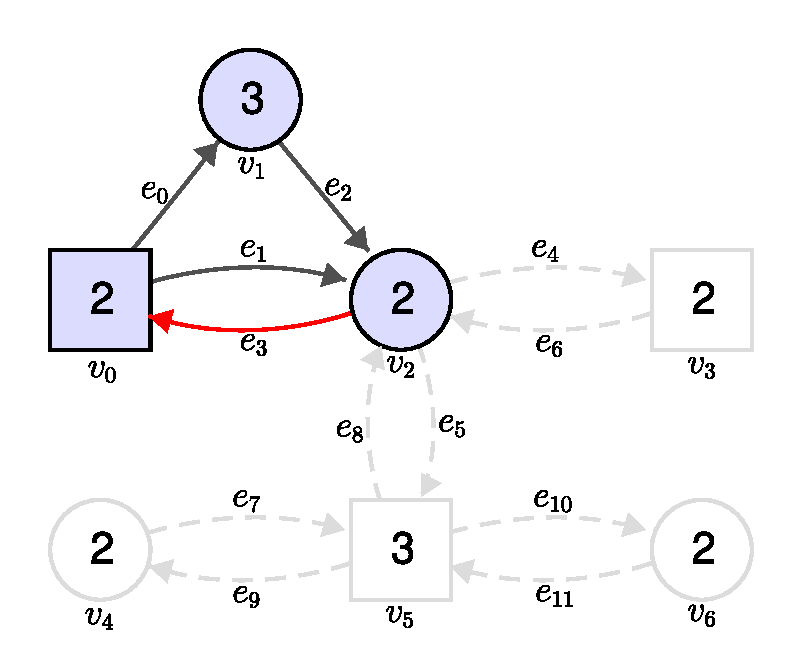
\includegraphics[width=\textwidth]{images/game02a}
        \caption{Initial assignment}
        \label{fig:game02a}
    \end{subfigure}
    \begin{subfigure}[b]{0.35\textwidth}
        \centering
        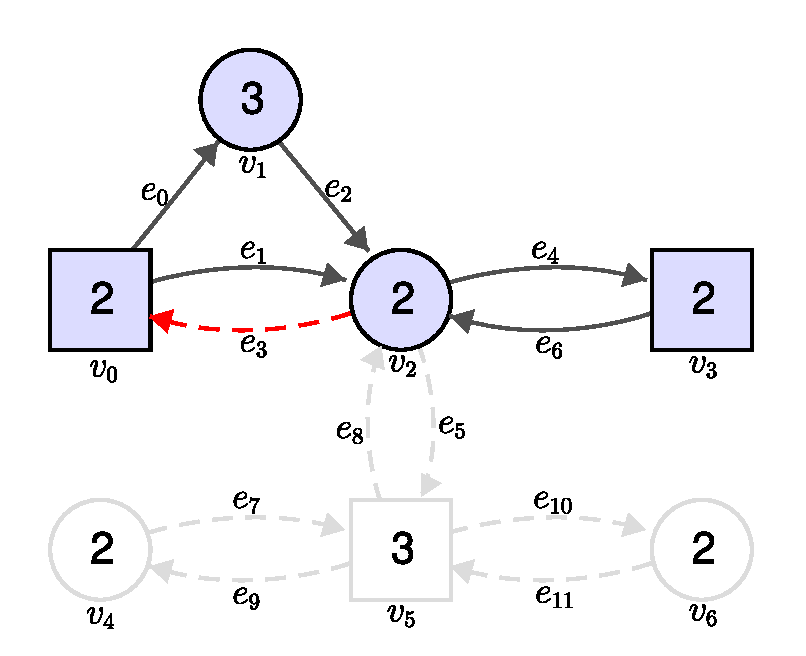
\includegraphics[width=\textwidth]{images/game02b}
        \caption{Satisfiable assignment}
        \label{fig:game02b}
    \end{subfigure}
    \caption{A parity game with vertices $\{v_0 \dots v_6\}$, edges $\{e_0 \dots e_{11}\}$, and priorities $\{2,3\}$. Dashed edges are unassigned. The red edge $e_3$ closes a cycle won by Player~$\odd$: in (a) it is part of the conflicting assignment, and in (b) it has been falsified by the propagator.}
    \label{fig:game02}
\end{figure}

Stronger versions of the $\mathcal{C}_{\noc}$ constraint can filter out assignments that necessarily lead to cycles with an odd maximum priority. For instance, if the former assignment had been considered first, the constraint could have determined in advance that $\mathcal{E}_3$ \textit{must} be $\bot$, since otherwise an odd cycle would be present.

\subsection{A No-Opponent-Cycle checker} \label{sec:nocchecker}
To enforce $\mathcal{C}_{\noc}$, we propose a checker based on recursively decomposing the graph into Strongly Connected Components (SCCs). By definition, all vertices inside an SCC of size greater than 1 are part of at least one cycle, while single-vertex SCCs may still contain self-loops.
%
Each resulting subgraph is then evaluated: if it contains a cycle in which the highest priority occurring infinitely often favors $\opponent$, the current assignment is rejected. Otherwise, the maximum priorities favouring $\player$ are removed from the SCC, and new SCCs are computed on the reduced graph.
%
If, in the end, no remaining single vertex has a self-loop with an $\opponent$ priority, the assignment is accepted.

\begin{algorithm}[htb]
\small
\caption{\textbf{\textit{NOCChecker}}}
\textbf{Input}: Current game graph $G$ \\
\textbf{Output}: $\top$ is valid; $\bot$ otherwise
\begin{algorithmic}[1]
    \FOR{$scc \in \textit{Tarjan}(G)$} \label{alg:noc-checker:breakingdown}
        \IF{$|scc| = 1$} \label{alg:noc-checker:single}
            \STATE $v \gets$ the unique vertex in $scc$
            \STATE \textbf{if }$\Omega(v) \bmod 2 = \opponent \land (v,v) \in E \land \mathcal{E}[(v,v)] = \top$ \textbf{then return $\bot$} \label{alg:noc-checker:self}  
        \ELSE
            \STATE $bestSet \gets \textit{bestVertices}(scc)$ \label{alg:noc-checker:best}
            \STATE $v \gets$ an arbitrary vertex in $bestSet$
            \STATE \textbf{if }$\Omega(v) \bmod 2 = \opponent$ \textbf{then return $\bot$} \label{alg:noc-checker:opponent}  

            \STATE \textbf{if }not \textit{NOCChecker}($G \setminus bestSet$) \textbf{then return $\bot$} \label{alg:noc-checker:recursion}
        \ENDIF
    \ENDFOR
    \RETURN $\top$
\end{algorithmic}
\label{alg:noc-checker}
\end{algorithm}

Algorithm~\ref{alg:noc-checker} is implemented recursively, with an argument corresponding to the subgraph formed by the vertices and edges assigned $\top$. Before invoking the function, all variables are checked to ensure they are fixed. The function is invoked as $\textit{NOCChecker}(G_\top)$, where $G_\top = (\{ v \mid \mathcal{V}_v = \top \}, \{ e \mid \mathcal{E}_e = \top \})$. The current subgraph $G$ is decomposed into SCCs using Tarjan’s algorithm~\citep{Tarjan:1972}, so that each SCC is analyzed independently (line~\ref{alg:noc-checker:breakingdown}).
%
In each iteration, the algorithm checks whether the current SCC consists of a single vertex (line~\ref{alg:noc-checker:single}). If so, it verifies whether the vertex has a self-loop and whether its priority matches that of $\opponent$; in such a case, the assignment is rejected (line~\ref{alg:noc-checker:self}).
%
If the SCC contains more than one vertex, the algorithm identifies the set of vertices with the highest priority (line~\ref{alg:noc-checker:best}) and selects one arbitrarily to check its parity. If the selected vertex’s priority corresponds to $\opponent$, the assignment is also rejected (line~\ref{alg:noc-checker:opponent}). Otherwise, the vertices in this highest-priority set are removed from the SCC, and the function is recursively called on the resulting subgraph (line~\ref{alg:noc-checker:recursion}).

The complexity of the \nocchecker propagator is polynomial in the size of the input graph. Each call to Tarjan's algorithm computes the SCCs in linear time, i.e., $\mathcal{O}(|V| + |E|)$. In the worst case, the algorithm may recursively remove and reprocess subsets of vertices with maximal priority multiple times. However, each vertex can only be part of a highest-priority set and removed once per recursive level, ensuring that the total number of Tarjan calls remains linear in the number of vertices. As a result, the overall time complexity of the propagator remains $\mathcal{O}(|V| \cdot (|V| + |E|))$ in the worst case.

\subsection{An Eager No-Opponent-Cycle Propagator} \label{sec:nocfilter}
In addition to \nocchecker, we also propose a complete propagator based on Depth-first Search (DFS) to explore the arena. The resulting DFS tree captures all possible paths from $v_0$, and can be used to detect all existing cycles. We define the propagator in the context of a \textit{Lazy Clause Generation} solver~\citep{DBLP:journals/constraints/OhrimenkoSC09}, to take advantage of the strong performance of this type of solver, in particular for problems that contain a large number of Boolean clauses. Algorithm~\ref{alg:noc-eager} presents this version of the propagator, which checks for cycles and reports failure if a cycle with highest priority in favour of $\opponent$ is detected.

\begin{algorithm}[htb]
\small
\caption{\textbf{\textit{NOCEager}}}
\textbf{Input}: Vertex list $path_V$,\ Edge list $path_E$,\ Current vertex $v$,\ Current edge $e$,\ Edge variables $\mathcal{E}$,\ Flag $\textit{defined}$ \\
\textbf{Output}: $\top$ is valid; $\bot$ otherwise
\begin{algorithmic}[1]
    \IF{$v \in path_V$} \label{alg:noc-eager:pathcheck}
        \STATE $i_v \gets \textit{index}(v, path_V)$
        \STATE $m \gets \max\{\Omega(v') \mid v' \in path_V[i_v:]\}$
        \IF{$m \bmod 2 = \opponent$} \label{alg:noc-eager:checkopponent}
            \STATE $\textit{reason} \gets \textit{clausify}(\neg path_E)$ \label{alg:noc-eager:reason}
            \STATE \textbf{if }not ($\mathcal{E}[e] \gets (\bot, \textit{reason}))$ \textbf{then return $\bot$}
        \ENDIF
    \ELSIF{$\textit{defined}$} \label{alg:noc-eager:defcheck}
        \FOR{$e' \in \textit{edges}(v) \textbf{ where } \mathcal{E}[e'] \ne \bot$} \label{alg:no-opponent-cycle-f1:edgecheck}
            \STATE $p_V \gets path_V \cup \{v\}$
            \STATE $p_E \gets path_E \cup \{e'\}$
            \STATE $w \gets \textit{target}(e')$
            \STATE $\textit{def} \gets \mathcal{E}[e'] = \top$
            \STATE \textbf{if }not \textit{NOCEager}(
                $p_V$,
                $p_E$,
                $w$,
                $e'$,
                $\mathcal{E}$,
                $\textit{def}$\ ) \textbf{then return $\bot$}
        \ENDFOR
    \ENDIF
    \RETURN $\top$
\end{algorithmic}
\label{alg:noc-eager}
\end{algorithm}

Algorithm~\ref{alg:noc-eager} is also written in a recursive style. The arguments $\mathit{path}_V$ and $\mathit{path}_E$ represent the currently explored path in the DFS procedure, expressed in terms of both vertices and edges. The parameter $v$ denotes the current vertex, $e$ is the currently explored edge, and $\mathcal{E}$ is the array of Boolean variables associated with the edges of the graph. The \noc propagator invokes this function as $\textit{NOCEager}(\emptyset,\ \emptyset,\ v_0,\ -1,\ \mathcal{E},\ \top)$, where $-1$ indicates that no edge has been selected yet from $\mathcal{E}$, as valid edges are indexed with $e \geq 0$.

First, consider the case where the current vertex $v$ is not already in the current path (i.e., the else case in line~\ref{alg:noc-eager:defcheck}). This indicates that no cycle has been detected so far, and the algorithm recursively explores each outgoing edge from $v$ whose value is not $\bot$, extending the path accordingly. A basic implementation of \noceager would only explore edges for which $\mathcal{E}[e'] = \top$, thus limiting the search to assigned edges. However, the goal of this propagator is to allow the exploration of at most one unassigned edge, in order to proactively eliminate potential cycles before they become committed.

In contrast, if the current vertex $v$ has appeared in the path (line~\ref{alg:noc-eager:pathcheck}), this implies that the current edge closes a cycle. The algorithm then determines the highest priority among the vertices in the cycle, and if this priority favors $\opponent$ (line~\ref{alg:noc-eager:checkopponent}), the current edge is set to $\bot$. If the edge had already been assigned $\top$, this causes a conflict and triggers backtracking.

Since Lazy Clause Generation (LCG) solvers require a justification for each propagation step (to enable clause learning), all edges in the detected cycle are collected to form a clause stating that at least one must be assigned $\bot$ (line~\ref{alg:noc-eager:reason}). For instance, in the scenario shown in Figure~\ref{fig:game02b}, the clause $(\neg \mathcal{E}_0 \vee \neg \mathcal{E}_2 \vee \neg \mathcal{E}_4 \vee \neg \mathcal{E}_6 \vee \neg \mathcal{E}_3)$ is generated as the reason for $\mathcal{E}_3 = \bot$ to prevent the opponent cycle.

The complexity \noceager is primarily driven by the DFS traversal over the graph, with additional work performed when a cycle is detected. In the worst case, the algorithm explores every simple path in the graph starting from the initial vertex. This may result in an exponential number of recursive calls in the number of vertices since each branching decision adds a new path to explore. However, in practice, the number of recursive calls is bounded by the number of edges assigned to $\top$ and at most one unassigned edge, significantly reducing the branching factor. Each recursive call performs a constant number of operations, except when a cycle is found (line~\ref{alg:noc-eager:pathcheck}). Nevertheless, because the algorithm may visit multiple paths and cycles, and because each edge can potentially trigger multiple clause generation steps before being fixed, the overall worst-case complexity remains exponential in the size of the graph. This trade-off is justified by the early pruning capabilities enabled by detecting potentially winning opponent cycles before they are fully formed, especially in graphs with many unassigned edges. In typical solver applications, where assignments propagate quickly and many edges are fixed early, the practical runtime of the propagator is significantly better than the theoretical worst case—as demonstrated by the experimental results presented in section \ref{sec:experiments}, where this approach consistently outperforms alternatives in both speed and effectiveness.

\subsection{Improved Filtering Strategy for the No-Opponent-Cycle Propagator}

In order to mitigate the exponential behavior of \noceager, we have developed a variant that memorizes cycles and can quickly remove some new cycles. To do so, one can use Algorithm \ref{alg:noc-memo}, which incorporates a parameter $\textit{memo}$ that stores, for each edge, the starting node of an infinite path and the associated highest priority. This information is updated whenever a cycle is found (line~\ref{alg:noc-memo:update}). If $\textit{memo}$ does not contain information about the next edge $e'$, or a new highest priority was found, then the propagator proceeds recursively as before (lines~\ref{alg:noc-memo:check1} and \ref{alg:noc-memo:check2}). Otherwise, it uses the stored information for the new edge (line~\ref{alg:noc-memo:reuse}). 
This results in polynomial worst-case runtime, since the recursion is now bounded by the number of edges and the number of different priorities. However, the memoization only captures cycles with the same starting node. The propagator may therefore miss some cycles, rendering it incomplete. To preserve completeness, this variant is therefore used in conjunction with the \nocchecker introduced earlier.

For the example of Figure \ref{fig:game02}, the updated version of \noc stores a tuple $(v=5, m=3)$ on edge $e_5$, indicating that the best priority reachable from this edge is 3 and that the infinite path starts at $v_5$. This prevents the exploration of the subgraph $\{v_4, v_5, v_6\}$ in future stages.
%
Remembering cycles is particularly effective in games where the number of cycles favoring $\player$ exceeds those favoring $\opponent$, as demonstrated below in the section on experiments.

\begin{algorithm}[htb]
\caption{\textbf{\textit{NOCMemo}}}
\small
\textbf{Input}: Vertex list $path_V$,\ Edge list $path_E$,\ Current vertex $v$,\ Current edge $e$,\ Edge variables $\mathcal{E}$,\ Flag $\textit{defined}$,\ Edge table $\textit{memo}$ \\
\textbf{Output}: $\top$ is valid; $\bot$ otherwise
\begin{algorithmic}[1]
    \IF{$v \in path_V$}
        \STATE $i_v \gets$ \textit{index}$(v,\ path_V)$
        \STATE $m \gets \max\{\Omega(v') \mid v' \in path_V[i_v:]\}$
        \STATE $\textit{memo}[e] \gets (v,\ m)$ \label{alg:noc-memo:update}
        \IF{$m \bmod 2 = \opponent$} 
            \STATE $\textit{reason} \gets \textit{clausify}(\neg path_E)$
            \STATE \textbf{if }not ($\mathcal{E}[e] \gets (\bot, \textit{reason}))$ \textbf{then return $\bot$}
        \ENDIF
    \ELSIF{$\textit{defined}$}
        \FOR{$e' \in \textit{edges}(v)\ \textbf{where}\ \mathcal{E}[e'] \ne \bot$}
            \STATE $(v_{memo},\ m_{memo}) \gets \textit{memo}[e']$

            \STATE $p_V \gets path_V \cup \{v\}$
            \STATE $p_E \gets path_E \cup \{e'\}$
            \STATE $w \gets \textit{target}(e')$
            \STATE $\textit{def} \gets \mathcal{E}[e'] = \top$

            \IF{$(v_{memo}, m_{memo}) = (-1, -1)$}
                \STATE \textbf{if }not \textit{NOCMemo}($p_V, p_E, w, e', \mathcal{E}, def , \textit{memo}$) \textbf{then return $\bot$} \label{alg:noc-memo:check1}
            \ELSE
                \STATE $i_v \gets \textit{index}(v_{memo},\ path_V)$
                \STATE $m \gets \max\{\Omega(v') \mid v' \in path_V[i_v:]\}$
                \IF{$m  > m_{memo}$}
                    \STATE \textbf{if }not \textit{NOCMemo}($p_V, p_E, w, e', \mathcal{E}, def , \textit{memo}$) \textbf{then return $\bot$} \label{alg:noc-memo:check2}
                \ELSE
                    \STATE $\textit{memo}[e] \gets \textit{memo}[e']$ \label{alg:noc-memo:reuse}
                \ENDIF
            \ENDIF
        \ENDFOR
    \ENDIF
    \RETURN $\top$
\end{algorithmic}
\label{alg:noc-memo}
\end{algorithm}

The three versions of the \noc propagator can be used to solve parity games, with \nocmemo requiring the \nocchecker.

\subsection{Solving for $\player$ and $\opponent$ in Parallel}\label{sec:parallel}

As our experiments will demonstrate, solver performance is heavily dependent on the game's underlying structure. A key observation is the asymmetry in computational cost inherent in game structure: properties that challenge $\player$'s solution often simplify $\opponent$'s, and vice versa. This problem duality allows us to transform and simplify the solution. By exploiting this, we can avoid a worst-case scenario for one player by solving the game from the opposite perspective. Consequently, solving the game from both perspectives in parallel significantly improves overall efficiency. This acceleration is largely attributed to the \noc propagator's capacity to rapidly prune the search space by eliminating $\opponent$'s winning options, effectively proving $\player$ has no winning strategy. We execute both perspectives concurrently and use the result obtained by the faster computation.

\begin{example}\label{exa:parallel}
Consider solving the parity game instance \texttt{cliquegame-2000.gm} from two different initial positions, node $0$ and node $123$:

\begin{verbatim}
nocq --gm cliquegame-2000.gm --init 0 --noc-even --print-time --print-sat
35.2712 EVEN (SAT)

nocq --gm cliquegame-2000.gm --init 0 --noc-odd --print-time --print-sat
0.03481 EVEN (UNSAT)

nocq --gm cliquegame-2000.gm --init 123 --noc-even --print-time --print-sat
0.0362277 ODD (UNSAT)

nocq --gm cliquegame-2000.gm --init 123 --noc-odd --print-time --print-sat
36.4283 ODD (SAT)
\end{verbatim}

\noindent
In Example~\ref{exa:parallel}, we observe a dramatic runtime asymmetry between the two perspectives:
\begin{itemize}
    \item \textbf{Initial node $0$:} Proving directly that \even has a winning strategy takes $\approx 35.27$\,s (\texttt{SAT}). In contrast, checking the complementary perspective for \odd determines that \odd has no winning strategy in just $0.035$\,s (\texttt{UNSAT}), indirectly proving \even's victory.
    \item \textbf{Initial node $123$:} The reverse occurs. Proving directly that \odd wins takes $\approx 36.43$\,s (\texttt{SAT}), whereas refuting \even's winning strategy takes only $0.036$\,s (\texttt{UNSAT}).
\end{itemize}
By launching both queries concurrently in parallel, the winning player is determined by the fastest terminating query (the \texttt{UNSAT} run) in under $0.04$\,s in both instances—achieving an empirical speedup of nearly three orders of magnitude.
\end{example}

In contrast, as confirmed by additional experiments, specialised solvers such as Oink and \zra compute the winning regions of both players simultaneously, so there is no analogous choice of perspective for them to exploit.

\subsection{The Integer Formulation (\nooppc-Int)}\label{sec:noc_int}

Definition~\ref{def:csp} introduces a Boolean encoding of the arena, enabling straightforward implementation via state-of-the-art SAT solvers, where constraints $\mathcal{C}_{v_0}, \mathcal{C}_{\player}, \mathcal{C}_{\opponent}$, and $\mathcal{C}_{E}$ are naturally expressed as clauses. Furthermore, modern SAT solvers such as CaDiCaL provide external propagator interfaces to implement $\mathcal{C}_{\noc}$ \citep{Fazekas:2023}.

However, to leverage higher abstraction level filtering algorithms (e.g., maintaining bounds consistency) in CP solvers, we extend this formulation to an integer-based model. The variable structure and constraint logic remain identical to Definition~\ref{def:csp}, with the following updates:

\paragraph{Variable Domains.} The variable set $\mathcal{X}$ defines a decision variable $\mathcal{V}_v$ for each node $v \in V$ over an integer domain $\mathcal{D}_{\mathbb{Z}}(v)$, where $0$ indicates that a vertex is inactive ($\bot$). Specifically:
\[
\mathcal{D}_{\mathbb{Z}}(v) = 
\begin{cases} 
    \{0, \dots, d_v\} & \text{if } v \in V_{\player}, \text{ where } \mathcal{V}_v = i > 0 \text{ selects the } i\text{-th successor } vE[i], \\
    \{0, 1\} & \text{if } v \in V_{\opponent}, \text{ where } 1 \text{ denotes that every successor is selected,}
\end{cases}
\]
where $d_v = |vE|$ represents the out-degree of vertex $v$.

A key advantage of the integer formulation is the unification of node activation and outgoing edge selection into a single decision. For player vertices ($v \in V_{\player}$), the domain value $\mathcal{V}_v = i$ directly encodes the selected successor edge $(v, vE[i])$. For opponent vertices ($v \in V_{\opponent}$), the Boolean flag $\mathcal{V}_v = 1$ inherently implies that all outgoing edges are active. This reduces the total number of variables from $\mathcal{O}(|V| + |E|)$ to strictly $\mathcal{O}(|V|)$, drastically shrinking the solver's search space and the number of constraint clauses.

\paragraph{Constraint Updates.} 
By leveraging the integer domain encoding, edge variables are eliminated. The original constraint $\mathcal{C}_{\player}$ ($\sum \mathcal{E}_{(v,w)} = 1$) is subsumed by domain construction, while edge-to-vertex reachability ($\mathcal{C}_{E}$) is folded directly into $\mathcal{C}_{\player}$ and $\mathcal{C}_{\opponent}$:

\begin{itemize}[leftmargin=3.0cm, labelwidth=2.8cm, align=right, itemsep=1.0ex, parsep=0pt]

    \item [$\mathcal{C}_{v_0}$ :] $\mathcal{V}_{v_0} > 0$

    \item [$\mathcal{C}_{\player}$ :] $\bigwedge_{v \in V_{\player}} \bigwedge_{i=1}^{d_v} \left( (\mathcal{V}_v = i) \rightarrow (\mathcal{V}_{vE[i]} > 0) \right)$

    \item [$\mathcal{C}_{\opponent}$ :] $\bigwedge_{v \in V_{\opponent}} \left( \mathcal{V}_v > 0 \rightarrow \bigwedge_{w \in vE} \mathcal{V}_w > 0 \right)$

    \item [$\mathcal{C}_{\noc}(f)$ :] $\bigwedge_{u_0, \dots, u_k} \left( \left( \bigwedge_{i=0}^{k-1} \text{Active}(u_i, u_{i+1}) \right) \to \bigwedge_{j=0}^{k-1} ((u_j = u_k) \to f(u_j, \dots, u_k)) \right)$

\end{itemize}
\noindent where the edge activation predicate $\text{Active}(v, w)$ for $w \in vE$ is defined as:
\[
\text{Active}(v, w) \equiv 
\begin{cases} 
    \mathcal{V}_v = \text{idx}_v(w) & \text{if } v \in V_{\player} \\
    \mathcal{V}_v > 0 & \text{if } v \in V_{\opponent}
\end{cases}
\]
\noindent where $\text{idx}_v(w) \in \{1, \dots, d_v\}$ denotes the unique index of successor $w$ in $vE$ (i.e., $vE[\text{idx}_v(w)] = w$).

\begin{figure}
    \centering
    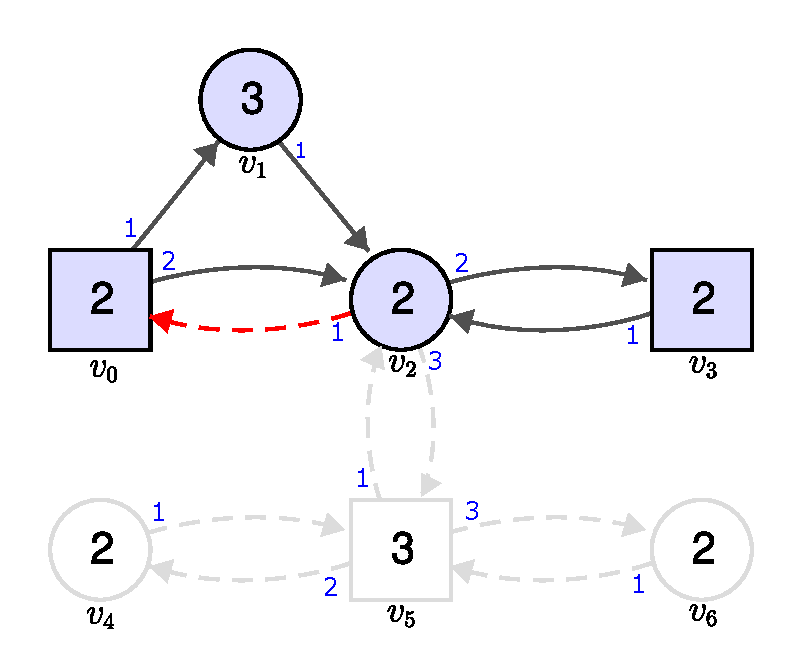
\includegraphics[width=0.35\textwidth]{images/game03.pdf}
    \caption{Integer variable representation of the search state from Example~\ref{exa:jurd-2-1-f0}. Domain values $\mathcal{V}_v = i$ directly designate the selected $i$-th successor $vE[i]$ for player vertices.}
    \label{fig:game03}
\end{figure}

\paragraph{Revisiting Example~\ref{exa:jurd-2-1-f0} under Integer Variables.}
To illustrate the difference in variable representation, consider the assignments described in Example~\ref{exa:jurd-2-1-f0} and Figure~\ref{fig:game03}.  In the \textit{Boolean/SAT formulation}, the initial failing search state required assigning seven distinct Boolean variables: three vertex variables ($\mathcal{V}_0 = \mathcal{V}_1 = \mathcal{V}_2 = \top$) and four explicit edge variables ($\mathcal{E}_0 = \mathcal{E}_1 = \mathcal{E}_2 = \mathcal{E}_3 = \top$).  In the \textit{Integer formulation}, the explicit edge variables ($\mathcal{E}_e$) are eliminated entirely. Since $v_0$ is an opponent vertex, $\mathcal{V}_0 = 1$ activates all its outgoing edges, while for player vertices the value selects the successor following the edge labels in Figure~\ref{fig:game03} (e.g., $\mathcal{V}_2 = 1$ selects $e_3$). The same initial state is thus encoded using only three vertex domain assignments:
\[
    \mathcal{V}_0 = \textcolor{blue}{1}, \quad \mathcal{V}_1 = \textcolor{blue}{1}, \quad \mathcal{V}_2 = \textcolor{blue}{1}
\]
Similarly, the second (satisfiable) assignment—which previously required setting 9 Boolean variables ($\mathcal{V}_0, \dots, \mathcal{V}_3$ and $\mathcal{E}_0, \mathcal{E}_1, \mathcal{E}_2, \mathcal{E}_4, \mathcal{E}_6$)—is now completely captured by assigning just four integer vertex variables:
\[
    \mathcal{V}_0 = \textcolor{blue}{1}, \quad \mathcal{V}_1 = \textcolor{blue}{1}, \quad \mathcal{V}_2 = \textcolor{blue}{2}, \quad \mathcal{V}_3 = \textcolor{blue}{1}
\]

The integer model replaces redundant edge choices with direct index selections, reducing both the number of active decision variables and the depth of the search tree.

\begin{algorithm}[htb]
\small
\caption{\textbf{\textit{NOCEagerInt}}}
\textbf{Input}: Vertex list $path_V$,\ Current vertex $v$,\ Former vertex $\textit{last}$,\ Flag $\textit{defined}$ \\
\textbf{Output}: $\top$ is valid; $\bot$ otherwise
\begin{algorithmic}[1]
    \IF{$v \in path_V$} \label{alg:noc-eager-int:pathcheck}
        \STATE $i_v \gets \textit{index}(v, path_V)$
        \STATE $m \gets \max\{\Omega(v') \mid v' \in path_V[i_v:]\}$
        \IF{$m \bmod 2 = \opponent$} \label{alg:noc-eager-int:checkopponent}
            \STATE $\textit{reason} \gets \textit{clausify}(\neg path_V)$ \label{alg:noc-eager-int:reason}

            \IF{$\textit{owner}(last)=\player$} \label{alg:noc-eager-int:filtering}
            \STATE $index \gets \textit{idx}_{\textit{last}}(v)$
            \STATE \textbf{if }not ($\mathcal{V}_{\textit{last}} \gets (\neq index, \textit{reason}))$ \textbf{then return $\bot$} \label{alg:noc-eager-int:filtering-player}
            \ELSE
                \STATE \textbf{if }not ($\mathcal{V}_{\textit{last}} \gets (0, \textit{reason}))$ \textbf{then return $\bot$} \label{alg:noc-eager-int:filtering-opponent}
            \ENDIF
        \ENDIF
    \ELSIF{$\textit{defined}$} \label{alg:noc-eager-int:defcheck}
        \IF{$\textit{owner}(v)=\player$}
            \STATE $\textit{targetSet} \gets \{vE[\mathcal{V}_v]\}$ \label{alg:noc-eager-int:traversal-player}
        \ELSE
            \STATE $\textit{targetSet} \gets vE$ \label{alg:noc-eager-int:traversal-opponent}
        \ENDIF

        \FOR{$w \in \textit{targetSet}$} \label{alg:noc-eager-int:edgecheck}
            \STATE $p_V \gets path_V \cup \{v\}$
            \STATE $\textit{def} \gets \mathcal{V}[w] > 0$ \label{alg:noc-eager-int:def}
            \STATE \textbf{if }not \textit{NOCEagerInt}(
                $p_V$,
                $w$,
                $v$,
                $\textit{def}$\ ) \textbf{then return $\bot$}
        \ENDFOR
    \ENDIF
    \RETURN $\top$
\end{algorithmic}
\label{alg:noc-eager-int}
\end{algorithm}

\paragraph{\nooppc Updated:}

Algorithm~\ref{alg:noc-eager-int} updates the eager propagator (\textit{NOCEager}) to operate directly over integer vertex domains ($\mathcal{V}$), eliminating all references to explicit edge variables ($\mathcal{E}$). The core modifications from Algorithm~\ref{alg:noc-eager} focus on conflict propagation and path exploration:

When an illegal opponent cycle is detected, conflict clauses are framed over vertex variables ($\neg path_V$) rather than edge variables ($\neg path_E$). Instead of setting a single Boolean edge variable to false ($\mathcal{E}[e] \gets \bot$), propagation directly prunes the domain of the predecessor vertex $\textit{last}$ based on its owner where for vertices controlled by $\player$ the propagator prunes only the specific index corresponding to the offending successor ($\mathcal{V}_{\textit{last}} \neq \textit{idx}_{\textit{last}}(v)$) (Line~\ref{alg:noc-eager-int:filtering-player}), leaving other outgoing choices open. For opponent vertices, it invalidates the whole outgoing successor vertex, setting $\mathcal{V}_{\textit{last}} \gets 0$ (Line~\ref{alg:noc-eager-int:filtering-opponent}).

Furthermore, instead of iterating over all non-false outgoing edges $e' \in \textit{edges}(v)$, line~\ref{alg:noc-eager-int:defcheck} constructs a candidate successor set ($\textit{targetSet}$) based on node ownership:
For player nodes ($v \in V_{\player}$), traversal is restricted solely to the single successor $vE[\mathcal{V}_v]$ designated by the integer variable (Line~\ref{alg:noc-eager-int:traversal-player}) and for opponent nodes ($v \in V_{\opponent}$), the algorithm branches across all outgoing successors $vE$ (Line~\ref{alg:noc-eager-int:traversal-opponent}).

Additionally, vertex assignment status ($\textit{def}$) is determined by verifying whether the target node is active ($\mathcal{V}[w] > 0$), replacing the Boolean edge evaluation ($\mathcal{E}[e'] = \top$) (Line~\ref{alg:noc-eager-int:def}).

\subsection{Search Strategies and Game-Specific Heuristics}\label{sec:search_heuristics}

Standard general-purpose search heuristics (such as VSIDS or $\text{dom}/\text{wdeg}$) branch indiscriminately across all unassigned variables in the solver's model. In parity games, this leads to redundant decision-making on unreached graph components or opponent vertices where no strategy choice is required. To overcome this, we design a customized, reachability-guided branching strategy (\nocbrancher) that focuses decisions exclusively on active, player-controlled choices.

\paragraph{Player-Restricted Decision Scope.}

Strategy synthesis requires determining choices solely for the searching player $\player$. For the opponent $\opponent$, vertex activation is deterministic: once an opponent node is active, constraint propagation automatically enforces that all of its outgoing edges are active. Consequently, the solver does not need to make decision steps on $\opponent$ vertices, as their outgoing transitions are fully determined by propagation once paths are established.

Consequently, \nocbrancher redefines search termination (\textsf{finished}): search terminates as soon as all \emph{active} $\player$ choices are resolved.

\paragraph{Reachability-Guided Branching Mechanism.}
The brancher selects decision variables dynamically by following graph reachability top-down from active paths: 
%
Over \textit{Boolean Formulation} (see Algorithm~\ref{alg:brancher-bool}), edge decisions are strictly gated by vertex reachability. An outgoing edge $e \in \text{outs}(v)$ is eligible for branching if and only if its source player vertex $v \in V_{\player}$ has already been fixed as active ($\mathcal{V}_v = \top$). Unfixed outgoing edges $\mathcal{E}_e$ are then assigned sequentially. This prevents the solver from making arbitrary edge assignments in disconnected regions of the arena.
%
Over \textit{Integer Formulation} (see Algorithm~\ref{alg:brancher-int}), for player vertices $v \in V_{\player}$, decisions are made directly on the integer variable $\mathcal{V}_v$. The brancher scans candidate vertices and selects the first unfixed $\mathcal{V}_v$ whose inactive state $0$ has been pruned by reachability propagation ($\min(\mathcal{D}(\mathcal{V}_v)) > 0$). Assigning an integer value directly selects the successor edge $(v, vE[i])$, allowing reachability propagation to immediately activate target node domains before the next decision step.

\begin{algorithm}[htb]
\small
\caption{\textbf{\textit{NOCBrancherBool}}}
\textbf{Input}: Game graph $G$, vertex variables $\mathcal{V}$, edge variables $\mathcal{E}$, target player $\player$ \\
\textbf{Output}: Decision variable $\mathcal{E}_e$ to branch on, or $\text{null}$ if finished
\begin{algorithmic}[1]
    \FOR{$v \in V$}
        \IF{$\textit{owner}(v) = \player \textbf{ and } \textit{isFixed}(\mathcal{V}_v) \textbf{ and } \mathcal{V}_v = \top$}
            \FOR{$e \in \textit{outs}(v)$}
                \IF{\textbf{not } $\textit{isFixed}(\mathcal{E}_e)$}
                    \RETURN $\mathcal{E}_e$
                \ENDIF
            \ENDFOR
        \ENDIF
    \ENDFOR
    \RETURN $\text{null}$
\end{algorithmic}
\label{alg:brancher-bool}
\end{algorithm}

\begin{algorithm}[htb]
\small
\caption{\textbf{\textit{NOCBrancherInt}}}
\textbf{Input}: Game graph $G$, vertex integer variables $\mathcal{V}$, target player $\player$ \\
\textbf{Output}: Decision variable $\mathcal{V}_v$ to branch on, or $\text{null}$ if finished
\begin{algorithmic}[1]
    \FOR{$v \in V$}
        \IF{$\textit{owner}(v) = \player \textbf{ and } \textbf{not } \textit{isFixed}(\mathcal{V}_v)$}
            \IF{$\min(\mathcal{D}(\mathcal{V}_v)) > 0$} 
                \RETURN $\mathcal{V}_v$
            \ENDIF
        \ENDIF
    \ENDFOR
    \RETURN $\text{null}$
\end{algorithmic}
\label{alg:brancher-int}
\end{algorithm}

By coupling decision variable selection directly with reachability, \nocbrancher ensures that search tree exploration constructs a memoryless winning strategy outward from $v_0$, drastically pruning irrelevant search subtrees.

\section{Experiments and Evaluation}\label{sec:experiments}

To evaluate our approach, we implemented our method based on \noc propagators using the Constraint Programming (CP) solver Chuffed (version 0.12.1)~\citep{chuffed:2018} and Google OR-Tools (version 9.15)~\citep{Perron:2024}. We used MiniZinc~\citep{DBLP:conf/cp/NethercoteSBBDT07} to model a CP baseline based on progress measures (Section~\ref{sec:cp-smt}).

For comparison, we employed several external state-of-the-art solvers: 
\begin{itemize}
    \item SAT Solvers (Reduction SAT): We used \textbf{CaDiCaL} (v2.1.3) \citep{Biere:Cadical:2024}, \textbf{MiniSat} (v2.2.0) \citep{Een:MiniSat:2003}, \textbf{Kissat} (v4.0.2) \citep{Biere:Kissat:2024}, and zChaff (v2007.3.12) \citep{Moskewicz:zChaff:2001}.
    \item CP and SMT Solvers (Progress Measure): We solved the MiniZinc progress-measure model with \textbf{Gecode}~\citep{Gecode:2019} and Google \textbf{CP-SAT}~\citep{Perron:2024}, and the SMT difference-logic encoding with \textbf{Z3} (v4.14.1.0)~\citep{deMoura:2008}.
    \item State-of-the-Art (SOTA) Parity Game Solvers: We incorporated Oink (fresh GitHub version) \citep{vanDijk:2018}, which includes several high-performance algorithms like Priority Promotion ($\textbf{PP}$ and $\textbf{PP+}$) and Parys' improvements ($\textbf{PAR}$). We also included the Zielonka Recursive Algorithm ($\textbf{ZRA}$), with an improved attractor strategy as detailed by \citet{Aggarwal:2023}, which offers better performance. 
\end{itemize}

All experiments were conducted on a benchmarking cluster with Intel Xeon 8260 CPUs (24 cores, non-hyperthreaded) with 268.55 GB of RAM, running Linux, however our Slurm execution scripts strictly limit each instance to 8 GB of RAM and 1 Core. The complete source code, including implementations and experimental setups, is available online~\citep{Hernandez:Github:NoOpponentCycle:2026}.

We evaluated all algorithms using a standard benchmark set commonly employed in parity game research, drawing from the PGSolver Library \citep{Friedmann:2017} and the Benchmarks for Parity Games \citep{Keiren:2015}. The games were classified into four categories:

\begin{itemize}
    \item Equivalence Checking (\textsf{EquivalenceCh}): This group contains 69 games derived from formal equivalence checking problems, including strong bisimulation, weak bisimulation, and stuttering equivalence. These games are characterized by complex, structured connectivity patterns reflecting system design.
    \item Model Checking (\textsf{ModelCh}): This set consists of 90 games originating from temporal logic model checking ($\mu$-calculus) against system models. These instances are considered organic and reflect real-world verification challenges.
    \item PGSolver Collection (\textsf{PGSolver}): This collection comprises 76 games sourced from the hardest known families of parity games, including ladder games, recursive ladder games, elevator verification, clique games, steady games, and Jurdziński games \citep{Benerecetti:2016}, likely to expose some of the worst performance.
    \item Random Games (\textsf{RandomG}): This category includes 75 randomly generated games with varying sizes and priority distributions, designed primarily to test the general robustness and average-case performance of solving algorithms.
\end{itemize}

To evaluate both the feasibility of the SAT reduction on smaller instances and solver scalability on larger ones, we partitioned the benchmark sets into two distinct size categories based on maximum vertex count. The smaller set consists of instances with up to $\approx 10^6$ vertices for \textit{Equivalence Checking} / \textit{Model Checking} and $\approx 10^3$ for \textit{PGSolver} / \textit{Random Games}. The larger set evaluates scalability with up to $\approx 3.5 \times 10^7$ vertices for \textit{Equivalence Checking} / \textit{Model Checking} and $\approx 10^5$ for \textit{PGSolver} / \textit{Random Games}.


\subsection{Benchmarking against other state of the art algorithms}

\begin{table}[ht]
\centering

\caption{Performance of algorithms on small-scale instances (Max vertices: EquivalenceCh/ModelCh $\approx 10^6$, PGSolver/RandomG $\approx 10^3$). Average time is reported in seconds using PAR2 scoring with a 60s timeout.}

\setlength{\tabcolsep}{1.2mm}
{\small 
\begin{tabular}{l|rr|rr|rr|rr}
\toprule
\textbf{Algorithm} & \multicolumn{2}{c|}{\textbf{EquivalenceCh}} & \multicolumn{2}{c|}{\textbf{ModelCh}} & \multicolumn{2}{c|}{\textbf{PGSolver}} & \multicolumn{2}{c}{\textbf{RandomG}} \\
 & Time & Solved & Time & Solved & Time & Solved & Time & Solved \\
\midrule
Oink(PP)        & 0.645         & 33/33 & 0.305         & 57/57 & 0.007         & 23/23 &  0.001         & 25/25 \\
Oink(PP+)       & 0.644         & 33/33 & 0.305         & 57/57 & \textbf{0.007}& 23/23 &  0.001         & 25/25 \\
Oink(PAR)       & 0.541         & 33/33 & 0.277         & 57/57 & 0.036         & 23/23 &  0.001         & 25/25 \\
ZRA(ImpAttr)    & 0.539         & 33/33 & 0.266         & 57/57 & 0.154         & 23/23 & \textbf{0.001} & 25/25 \\
\rowcolor{gray!20}
\noc(Ours)      & \textbf{0.398}& 33/33 & \textbf{0.201}& 57/57 & 0.016         & 23/23 &  0.003         & 25/25 \\
SAT(CaDiCaL)    & 60.732        & 19/33 & 75.560        & 23/57 & 6.815         & 22/23 &  2.086         & 25/25 \\
SAT(Kissat)     & 113.050       &  2/33 & 79.001        & 21/57 & 6.064         & 22/23 &  2.628         & 25/25 \\
SAT(MiniSat)    & 79.766        & 17/33 & 79.639        & 22/57 & 6.491         & 22/23 &  2.806         & 25/25 \\
\bottomrule
\end{tabular}
}
\label{tab:smallgames}
\end{table}

Table~\ref{tab:smallgames} evaluates the performance of \noc against two primary baselines on small benchmark instances: (1) constraint-based approaches that reduce the problem to SAT (using CaDiCaL, Kissat, and MiniSat), and (2) specialized, non-constraint-based solvers, including the \zra algorithm (Improved Attractor) and various Oink configurations (PP, PP+, PAR).

Overall, \noc substantially outperforms all SAT-based methods, achieving up to two to three orders of magnitude speedup in PAR2 time while successfully solving $100\%$ of the benchmark instances (whereas SAT solvers fail on up to $94\%$ of the \textsf{EquivalenceCh} set). Furthermore, \noc demonstrates competitive performance against top-tier specialized algorithms: it achieves the fastest overall runtime on both the \textsf{EquivalenceCh} (0.398s) and \textsf{ModelCh} (0.201s) benchmarks, and remains well within a sub-20 millisecond range on \textsf{PGSolver} and \textsf{RandomG}—costing only a negligible fraction of a second over the fastest Oink variant.

\begin{table}[ht]
\centering
\caption{Performance of algorithms on large-scale instances (Max vertices: EquivalenceCh/ModelCh $\approx 3.5 \times 10^7$, PGSolver/RandomG $\approx 10^5$). Average time is reported in seconds using PAR2 scoring with a 60s timeout.}

\setlength{\tabcolsep}{1.2mm}
{\small 
\begin{tabular}{l|rr|rr|rr|rr}
\toprule
\textbf{Algorithm} & \multicolumn{2}{c|}{\textbf{EquivalenceCh}} & \multicolumn{2}{c|}{\textbf{ModelCh}} & \multicolumn{2}{c|}{\textbf{PGSolver}} & \multicolumn{2}{c}{\textbf{RandomG}} \\
 & Time & Solved & Time & Solved & Time & Solved & Time & Solved \\
\midrule
Oink(PP)        & 29.375         & 30/36 & 9.003         & 33/33 & 8.293         & 48/53 & 0.039         & 50/50 \\
Oink(PP+)       & 29.392         & 30/36 & 8.986         & 33/33 & 8.295         & 48/53 & \textbf{0.039}& 50/50 \\
Oink(PAR)       & 28.525         & 30/36 & 8.345         & 33/33 & 16.536        & 42/53 & 0.043        & 50/50 \\
ZRA(ImpAttr)    & \textbf{21.249}& 35/36 & 8.606         & 33/33 & 16.372        & 42/53 & 0.042         & 50/50 \\
\rowcolor{gray!20}
\noc(Ours)     & 22.049          & 36/36 & \textbf{7.719}& 33/33 & \textbf{7.984}& 52/53 & 0.383         & 50/50 \\
\bottomrule
\end{tabular}
}
\label{tab:biggames}
\end{table}

Table~\ref{tab:biggames} presents the evaluation on large-scale benchmark instances, assessing the scalability of \noc against \zra and the Oink solver suite. SAT-based methods are omitted from this comparison, as they failed to scale to these instance sizes within feasible resource limits. 

Overall, \noc exhibits superior scalability and solves the highest total number of instances across all benchmark suites ($171/172$). Crucially, on \textsf{EquivalenceCh}, \noc is the only method to solve all 36 instances while maintaining runtime performance competitive with \zra. On \textsf{ModelCh}, \noc achieves the best overall runtime ($7.719$\,s). On the \textsf{PGSolver} collection, \noc also delivers top performance, cutting runtimes by over $2\times$ compared to Oink(PAR) and \zra while solving $52/53$ instances (compared to $48/53$ for Oink PP/PP+). Finally, all solvers handle \textsf{RandomG} in under $0.4$ seconds; on this suite \noc is slower than the specialised solvers ($0.383$\,s vs.\ $0.039$\,s for Oink(PP)) but remains sub-second. Overall, these results show that constraint-based propagators can match or outperform dedicated solvers on massive instances with up to 35 million vertices.

The runtime metrics for the \noc and \zra approaches include both the solver execution time and the internal problem-preparation time (excluding I/O operations such as file reading). In contrast, for the SAT-based approaches we report only the solving time. This distinction is made because the preparation phase for the SAT-based methods—particularly the encoding generation—is substantially more expensive and was not a primary target of optimization in this work. 

\subsection{Comparison with CP and SMT encodings of the progress measure}\label{sec:cp-smt}

The comparison above covers SAT-based reductions. To complete the picture of constraint-based approaches, we also compare \noc against encodings that keep the progress measure but hand it to more expressive solvers: a MiniZinc CP model that expresses the progress measure using integer variables and constraints, solved by Gecode and CP-SAT, and the SMT model of Section~\ref{sec:smt} that implements the progress measure in difference logic, solved by Z3. In this experiment, \noc was run with the \nocmemo propagator in Chuffed, and all approaches solved the game from Player~$\even$'s perspective only; that is, \noc did not use the parallel search over both players' perspectives described in Section~\ref{sec:parallel}. We use Jurdziński games, which allow the size of the graph to be varied systematically: $J_{\ell,10}$ has 10 blocks and $\ell \in \{10, 20, \dots, 80\}$ levels.

\begin{table}[ht]
\centering
\caption{Solving time (in seconds) on Jurdziński games $J_{\ell,10}$ for \noc and for the progress-measure encodings solved by CP (MiniZinc with Gecode and CP-SAT) and SMT (Z3) solvers. A dash indicates a time exceeding 5 minutes.}
{\small
\begin{tabular}{r|rrrr}
\toprule
$\ell$ & \textbf{Chuffed}(\nocmemo) & \textbf{MiniZinc}(Gecode) & \textbf{MiniZinc}(CP-SAT) & \textbf{Z3} \\
\midrule
10 & \textbf{0.01} & 0.59   & 0.71   & 0.22   \\
20 & \textbf{0.02} & 3.06   & 2.59   & 0.58   \\
30 & \textbf{0.03} & 10.57  & 6.15   & 2.64   \\
40 & \textbf{0.05} & 28.53  & 12.52  & 7.76   \\
50 & \textbf{0.07} & 63.77  & 22.47  & 18.11  \\
60 & \textbf{0.10} & 126.88 & 37.41  & 35.76  \\
70 & \textbf{0.13} & 231.51 & 58.22  & 65.62  \\
80 & \textbf{0.17} & -      & 88.89  & 111.80 \\
\bottomrule
\end{tabular}
}
\label{tab:cp-cp}
\end{table}

Table~\ref{tab:cp-cp} shows that \noc outperforms all three progress-measure approaches by two to three orders of magnitude, and that the gap widens with the size of the game: at 80 levels, \noc needs $0.17$\,s, whereas CP-SAT needs $88.89$\,s, Z3 needs $111.80$\,s, and Gecode exceeds the 5-minute limit. Among the baselines, Z3 is the fastest on small games, but CP-SAT scales better beyond 60 levels. The progress-measure encodings are also expensive in memory: MiniZinc with Gecode used over 256\,GB to complete the larger instances, so, as in the memory experiment of Section~\ref{sec:memory}, these runs were not subject to the 8\,GB limit. Together with Table~\ref{tab:smallgames}, these results show that \noc outperforms SAT-, CP- and SMT-based encodings of the progress measure.

\subsection{Comparison between different versions of \noc}
\begin{table}[ht]
\centering
\caption{Performance comparison between Boolean and Integer encodings of \noc using Chuffed and OR-Tools. PTime is the preparation time and STime the solving time (in seconds). Bold values mark the lowest PTime and STime in each suite. Same configuration as Table~\ref{tab:biggames}.}
\setlength{\tabcolsep}{1.2mm}
{\small 
\begin{tabular}{cl|rrr|rrr|rrr|rrr}
\toprule
\multicolumn{2}{c|}{\textbf{Solver}} & \multicolumn{3}{c|}{\textbf{EquivalenceCh}} & \multicolumn{3}{c|}{\textbf{ModelCh}} & \multicolumn{3}{c|}{\textbf{PGSolver}} & \multicolumn{3}{c}{\textbf{RandomG}} \\
& & PTime & STime & Solved & PTime & STime & Solved & PTime & STime & Solved & PTime & STime & Solved \\
\midrule
\multirow{2}{*}{\rotatebox[origin=c]{90}{\textbf{Bool}}} 
& Chuffed & 21.936 & \textbf{ 0.113} & 36/36 
          &  7.689 & \textbf{ 0.030} & 33/33 
          &  3.006 & \textbf{ 4.978} & 52/53 
          &  0.289 & \textbf{ 0.094} & 50/50 \\
& ORTools & 41.576 & 28.391 & 36/36 
          & 14.472 & 13.246 & 32/33 
          &  3.578 & 43.513 & 34/53 
          &  0.296 &  3.027 & 49/50 \\
\midrule
\multirow{2}{*}{\rotatebox[origin=c]{90}{\textbf{Int}}} 
& Chuffed & \textbf{16.107} & 99.565 &  8/36 
          & \textbf{ 6.225} & 66.405 & 17/33 
          & \textbf{ 1.357} &  7.436 & 51/53 
          & \textbf{ 0.141} &  1.176 & 50/50 \\
& ORTools & 73.646 & 99.406 & 32/36 
          & 25.097 &  6.386 & 33/33 
          &  4.320 &  9.995 & 49/53 
          &  0.405 &  2.847 & 49/50 \\
\bottomrule
\end{tabular}
}
\label{tab:bool_int}
\end{table}

In the context of competitive parity game solving against state-of-the-art tools, the primary evaluation metric is the total execution time ($\textsf{TTime} = \textsf{PTime} + \textsf{STime}$). Our experimental evaluation proceeds in two phases: comparing the encoding paradigms and assessing the underlying solver engines.

With Chuffed, the Boolean formulation clearly outperforms the Integer encoding in solving tractability and overall coverage. On structured instances (\textsf{EquivalenceCh} and \textsf{ModelCh}), the Boolean model allows the solver to find solutions almost immediately ($\textsf{STime} < 0.12\,\text{s}$ with Chuffed). Conversely, the Integer model causes severe thrashing during search, driving Chuffed's $\textsf{STime}$ up to $99.565\,\text{s}$ and resulting in widespread timeouts. Although the Integer model reduces preparation overhead ($\textsf{PTime}$) for Chuffed by 19--55\%, this gain is small compared to the resulting penalty in search time. Consequently, with Chuffed the Boolean encoding provides the lowest end-to-end $\textsf{TTime}$.

The performance of the solvers depends heavily on the chosen encoding. Chuffed is clearly superior for the Boolean model, achieving faster compilation times and solving times between $8\times$ (\textsf{PGSolver}) and over $400\times$ (\textsf{ModelCh}) lower than OR-Tools (solving $171/172$ vs.\ $151/172$ instances). However, OR-Tools displays higher robustness over the Integer representation, successfully solving $163/172$ instances compared to Chuffed's $126/172$, and maintaining a low $\textsf{STime}$ of $6.386\,\text{s}$ on \textsf{ModelCh}. Nonetheless, because OR-Tools consistently introduces higher $\textsf{PTime}$ overhead, the combination of the \textbf{Boolean encoding with Chuffed} delivers the best overall competitive performance.

\def\sat#1{\sathelper#1\relax}
\def\sathelper#1 #2 #3\relax{%
  \textnormal{%
    \makebox[1.0em][r]{#1}$|$\makebox[1.0em][r]{#2}$|$\makebox[1.0em][l]{#3}%
  }%
}

\begin{table}[ht]
\centering
\caption{Performance comparison of \noc across three heuristic search strategies under Boolean and Integer encodings using Chuffed and OR-Tools. Same configuration as Table~\ref{tab:bool_int}.}

\setlength{\tabcolsep}{3.8pt}

\begin{tabular}{cc|l|rrr|rrr|rrr|rrr}
\toprule
\multicolumn{2}{c|}{\textbf{Solver}} & \textbf{Strategy} & 
        \multicolumn{3}{c|}{\textbf{EquivalenceCh}($N{=}36$)} & 
        \multicolumn{3}{c|}{\textbf{ModelCh}($N{=}33$)} & 
        \multicolumn{3}{c|}{\textbf{PGSolver}($N{=}53$)} & 
        \multicolumn{3}{c}{\textbf{RandomG}($N{=}50$)} \\
& & 
  & \multicolumn{1}{c}{\even} & \multicolumn{1}{c}{\odd} & \multicolumn{1}{r|}{\sat{S U T}} 
  & \multicolumn{1}{c}{\even} & \multicolumn{1}{c}{\odd} & \multicolumn{1}{r|}{\sat{S U T}} 
  & \multicolumn{1}{c}{\even} & \multicolumn{1}{c}{\odd} & \multicolumn{1}{r|}{\sat{S U T}} 
  & \multicolumn{1}{c}{\even} & \multicolumn{1}{c}{\odd} & \multicolumn{1}{r}{\sat{S U T}}  \\
\midrule
\multirow{6}{*}{\rotatebox[origin=c]{90}{\textbf{Boolean}}} 
& \multirow{3}{*}{\rotatebox[origin=c]{90}{Chuffed}} 
& ValMin  & 19 & 17 & \sat{0 36 0} 
          &  6 & 28 & \sat{0 33 0} 
          & 31 & 45 & \sat{2 50 1} 
          & 46 & 47 & \sat{5 45 0} \\

& & Reach   & \textbf{36} & \textbf{36} & \sat{0 36 0} 
            & \textbf{33} & \textbf{33} & \sat{0 33 0} 
            & \textbf{31} & \textbf{47} & \sat{3 49 1} 
            & 32 & 37 & \sat{0 49 1} \\
            
& & Rand    & 19 & 17 & \sat{0 36 0} 
            &  6 & 27 & \sat{0 33 0} 
            & 28 & 30 & \sat{1 36 16} 
            & \textbf{49} & \textbf{48} & \sat{3 47 0} \\

\cmidrule{2-15}
& \multirow{3}{*}{\rotatebox[origin=c]{90}{ORTools}} 
& ValMin    & 28 & 28 & \sat{0 36 0} 
            & 30 & 31 & \sat{0 32 1} 
            & \textbf{27} & 32 & \sat{0 34 19}
            & \textbf{46} & 38 & \sat{3 46 1} \\

& & Reach   & \textbf{36} & \textbf{36} & \sat{9 27 0} 
            & \textbf{32} & \textbf{32} & \sat{13 19 1}
            &         21  & \textbf{39} & \sat{7 39 7}
            & 16 & 34 & \sat{0 49 1} \\
            
& & Rand    & 13 & 12 & \sat{0 21 15}
            & 12 & 27 & \sat{0 31 2}
            & 25 & 28 & \sat{0 34 19}
            & 40 & \textbf{43} & \sat{3 46 1} \\
\midrule
\multirow{6}{*}{\rotatebox[origin=c]{90}{\textbf{Integer}}} 
& \multirow{3}{*}{\rotatebox[origin=c]{90}{Chuffed}} 
& ValMin    &  8 &  0 & \sat{0 8 28} 
            &  3 & 15 & \sat{0 17 16} 
            & 29 & \textbf{48} & \sat{3 48 2}
            & 47 & 46 & \sat{6 44 0} \\

& & Reach   & \textbf{ 9} & \textbf{ 9} & \sat{1 8 27} 
            & \textbf{22} & \textbf{22} & \sat{16 17 0}
            & 29 & 47 & \sat{9 41 3}
            & 32 & 37 & \sat{0 49 1} \\
            
& & Rand    &  8 &  1 & \sat{0 9 27}
            &  4 & 19 & \sat{0 23 10}
            & \textbf{31} & 32 & \sat{5 30 18}
            & \textbf{48} & \textbf{48} & \sat{4 46 0} \\

\cmidrule{2-15}
& \multirow{3}{*}{\rotatebox[origin=c]{90}{ORTools}} 
& ValMin    & 25 & 30 & \sat{0 32 4}
            & 31 & \textbf{32} & \sat{0 33 0} 
            & \textbf{27} & 47 & \sat{5 44 4}
            & \textbf{47} & \textbf{41} & \sat{3 46 1} \\

& & Reach   & \textbf{31} & \textbf{32} & \sat{6 26 4}
            & \textbf{33} & 31 & \sat{9 24 0}
            & 25 & \textbf{48} & \sat{8 42 3} 
            & 17 & 34 & \sat{0 49 1} \\
            
& & Rand    & 13 & 12 & \sat{0 21 15}
            & 16 & 26 & \sat{0 31 2} 
            & 27 & 28 & \sat{1 31 21}
            & 44 & 37 & \sat{2 46 2} \\
\bottomrule
\end{tabular}
\label{tab:branch_bool}
\end{table}

\subsection{Analysis of Search Strategies and Player Duality}
Table~\ref{tab:branch_bool} breaks down the parallel execution of \noc into its dual search threads ($\even$ and $\odd$) and details the terminal resolution status \textbf{Satisfiable | Unsatisfiable | Timeout} ($\textsf{S}|\textsf{U}|\textsf{T}$). Columns $\even$ and $\odd$ give the number of instances solved within the timeout by the thread searching from each player's perspective, while $\textsf{S}|\textsf{U}|\textsf{T}$ reports the outcome of the first thread to terminate.

\paragraph{Player Duality and UNSAT-Driven Resolution.}
Across all benchmark suites, problem resolution is overwhelmingly driven by unsatisfiability refutations ($\textsf{U}$) rather than direct satisfiable assignments ($\textsf{S}$). For instance, in \textsf{EquivalenceCh} and \textsf{ModelCh}, all completed instances under Boolean Chuffed are resolved exclusively through unsatisfiability proofs ($\textsf{U} = 36$ and $\textsf{U} = 33$, respectively, with $\textsf{S} = 0$). In two-player zero-sum parity games, establishing that one player cannot satisfy their winning condition immediately confirms the opponent's victory. Because refutation complexity varies depending on which player's winning condition is formulated, executing the $\even$ and $\odd$ perspectives in parallel ensures the solver terminates as soon as the faster UNSAT proof is established. Solvers equipped with lazy clause generation (such as Chuffed) exploit this asymmetry effectively by learning compact nogoods from conflict subtrees, yielding zero timeouts ($\textsf{T}{=}0$) across multiple benchmark sets.

\paragraph{Heuristic Specialization.}
The structural reachability heuristic (\textsf{Reach}) provides the highest per-thread consistency on structured benchmarks: with the Boolean encoding and Chuffed, both the $\even$ and $\odd$ threads solve all \textsf{EquivalenceCh} and \textsf{ModelCh} instances, whereas under \textsf{ValMin} and \textsf{Rand} each thread solves only part of them. Crucially, while refutation via unsatisfiability remains the predominant resolution pathway across all suites, the reachability heuristic significantly enhances the solver's ability to identify direct satisfying assignments ($\textsf{S}$). By guiding search decisions along feasible game transitions rather than relying on arbitrary value orderings, \textsf{Reach} constructs valid winning strategies far more effectively—evident in \textsf{EquivalenceCh} and \textsf{ModelCh} under OR-Tools, where SAT-derived solutions increase noticeably (e.g., reaching $\textsf{S} = 9$ and $\textsf{S} = 13$, compared to $\textsf{S} = 0$ under \textsf{ValMin}). Conversely, with Chuffed, randomized branching (\textsf{Rand}) yields the highest per-thread solved counts on unstructured topologies (\textsf{RandomG}), suggesting that it avoids pathological search traps in dense random graphs where topological reachability offers little guidance.

\subsection{Resource Utilization Analysis}\label{sec:memory}

A key motivation for developing the \noc propagator was to avoid the resource overhead associated with introducing the Boolean literals and clauses required for the progress measure variables and constraints. %In our experiments, 
We also evaluated the memory consumption of \noc compared to other methods. Unlike the runtime experiments, where each instance was limited to 8\,GB of RAM, for this experiment only we lifted the memory limit and allowed each solver to use the entire memory available on the node (268.55\,GB), so that the peak memory usage of the SAT-based approaches could be measured rather than truncated by the limit.

The results of these additional experiments are summarised in Figure~\ref{fig:peakofmemory}. While \noc requires at most 700MB of memory for games with 13 thousand vertices, and \zra up to 17MB, the SAT-based approaches consume significantly more. In particular, we see that CaDiCaL, MiniSat, and Kissat report memory usage exceeding 39~GB for the same instances.

\section{Games with Additional Constraints}

As we will see in this section, our method flexibly integrates additional constraints—such as quantitative or structural requirements—without any modification to the core algorithm. This inherent adaptability to various constraints is a decisive advantage over non-CP approaches, which necessitate custom adaptations for every additional set of constraints in the problem.

\begin{figure}
    \centering
    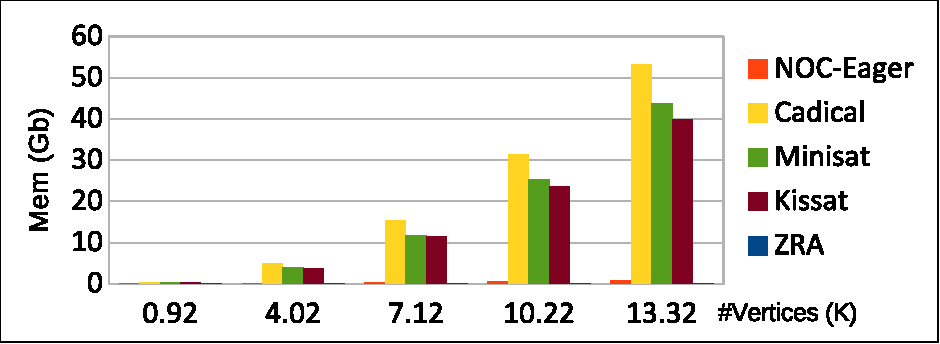
\includegraphics[width=0.7\textwidth]{images/peakmemory.pdf} 
    \caption{Memory usage in GB for solving  Jurdziński parity games (one of the hardest games in the PGSolver collection), constrained to 13 thousand vertices.}
    \label{fig:peakofmemory}
\end{figure}

\subsection{Automated Synthesis of Reactive Systems}

In (local) model checking, it suffices to determine the winner from a given vertex (satisfiable if won by Player~$\even$, unsatisfiable if won by Player~$\odd$). However, applications like automated synthesis~\citep{Bruyere:2022,Finkbeiner:2018,Luttenberger:2020} require explicit winning strategies, that is, a description of the decisions to be made by the winner at each vertex.

Our satisfiability encoding can capture multiple winning plays simultaneously. For instance, in Figure~\ref{fig:game02b}, a solution assigning $\top$ to vertices $\mathcal{V}_0$ to $\mathcal{V}_3$ and edges $\mathcal{E}_0$, $\mathcal{E}_1$, $\mathcal{E}_2$, $\mathcal{E}_4$, and $\mathcal{E}_6$ captures two distinct plays: $\langle e_0e_2e_4e_6 \rangle$ and $\langle e_1e_4e_6 \rangle$.
%
To extract individual winning plays, we extend the CSP with variables and constraints such that each solution corresponds to exactly one play. We define a sequence of integer variables $(\mathcal{P}_s)_{s \in \{0..\mid V \mid - 1\}}$ to represent the path. More specifically, we also add:
\begin{itemize}
\item $\mathsf{h}$: the position where the cycle (tail) starts, so that the finite prefix is $\mathcal{P}_0 \dots \mathcal{P}_{\mathsf{h}-1}$;

\item $\mathsf{t}$: the last position of the cycle.
\end{itemize} 

\noindent 
We then introduce three new constraints:
\begin{itemize}
\item ($\mathcal{C}_{\textit{path}}$): 
$\mathsf{t} \in \{0 \dots |V| -1\} \wedge \mathcal{P}_0 = v_0 \wedge \bigwedge_{s \in \{1..\mathsf{t}\}} \bigvee_{e=(v,w) \in E} (\mathcal{E}_e \wedge \mathcal{P}_{s-1} = v \wedge \mathcal{P}_s = w)$;
This ensures each step follows a valid edge;
\end{itemize}

\begin{itemize}
\item ($\mathcal{C}_{\textit{cycle}}$): 
$\mathsf{h} \in \{0 \dots \mathsf{t}\} \wedge \bigvee_{e=(v,w) \in E} (\mathcal{E}_e \wedge \mathcal{P}_\mathsf{t} = v \wedge \mathcal{P}_\mathsf{h} = w)$; \\
It ensures that an active edge leads from the last position $\mathsf{t}$ back to position $\mathsf{h}$, closing the cycle;
\end{itemize}

\begin{itemize}
\item ($\mathcal{C}_{\textit{unique}}$): 
$\bigwedge_{i \neq j \in \{0 \dots \mathsf{t}\}} (\mathcal{P}_i \neq \mathcal{P}_j)$; \\
This constraint enforces only one cycle.
\end{itemize} 

These constraints can be added in MiniZinc without modifying the core algorithm of \noc. Using Chuffed as the backend, we enumerate all solutions to obtain the set of winning plays, represented as vertex sequences. 

\subsection{Energy Conditions/Games}

We consider games with additional quantitative objectives. In \textit{Energy Games}~\citep{ChatterjeeD12}, each edge carries an energy level (a weight), and a play is winning if the running sum of these levels remains non-negative at all times, in addition to satisfying the parity condition.
%
This requirement can be encoded using the $\mathcal{P}$ variables introduced earlier. Given a set of energy levels $(L_e)_{e \in E}$, we define integer variables $(\mathcal{I}_s)_{s \in \{0..\mathsf{t} - \mathsf{h}\}}$ to represent the edges in the infinite cycle (tail) of the play:

\begin{itemize}
    \item $\mathcal{C}_{\textit{infEdges}} : \forall s \in \{0..\mathsf{t} - \mathsf{h}\} (\mathcal{I}_s = E(\mathcal{P}_{\mathsf{h}+s}, \mathcal{P}_{\mathsf{h}+((s+1) \bmod (\mathsf{t}-\mathsf{h}+1))}))$
\end{itemize}

We then impose the following constraint to ensure the total energy level in the cycle is non-negative:

\begin{itemize}
    \item $\mathcal{C}_{\textit{energy}} : \sum_{s=0}^{\mathsf{t}-\mathsf{h}} L_{\mathcal{I}_s} \geq 0$
\end{itemize}

While a complete model would also enforce energy constraints over all finite prefixes (up to $\mathsf{t}$), we omit these here for brevity. Note also that these constraints restrict the play selected by the $\mathcal{P}$ variables; requiring the energy condition on every play consistent with the strategy calls for a universal formulation, which we leave for future work. 

Many other extensions---such as multi-dimensional energy bounds and other quantitative payoff constraints---can be modelled similarly using additional constraints or objective functions~\citep{bozzelly:2020,Fijalkow:2014,Mogavero:2015,Weinert:2016}. Further work is needed to precisely define each requirement and establish the appropriate constraints.

\section{Conclusions}
We have introduced a novel constraint-based approach for parity games which does not require integer-based progress measures. The experiments show that our method significantly outperforms existing constraint-based approaches, reducing runtime by up to two orders of magnitude and peak memory by over 95\% on the Jurdziński games we measured, while remaining competitive against state-of-the-art specialized non-CP solvers. 

Our investigation into different modeling paradigms and search strategies highlights key trade-offs in constraint-based game solving. While the integer formulation substantially reduces the total variable count and compilation overhead by eliminating explicit edge variables, our empirical results demonstrate that the Boolean formulation coupled with Lazy Clause Generation provides superior solving tractability, enabling rapid nogood learning and immediate refutations. Furthermore, our customized reachability-guided branching heuristic (\nocbrancher) effectively confines the search space to active, player-controlled decisions, dramatically outperforming standard general-purpose variable selection on structured verification benchmarks, while randomized branching provides robustness on dense topologies. Exploiting player duality through concurrent bidirectional search proves crucial, consistently allowing the solver to terminate via the faster unsatisfiability proof.

Our key innovation—encapsulating cycle elimination within a specialized global constraint rather than a large static SAT encoding—not only improves performance but also provides a flexible framework that seamlessly accommodates additional structural and quantitative requirements, such as path extraction for reactive synthesis and energy constraints. This work demonstrates that constraint programming with domain-specific global propagators offers a practical, highly expressive, and computationally efficient foundation for modern formal verification tools.

% To print the credit authorship contribution details
\printcredits

\newpage

%% Loading bibliography style file
% \bibliographystyle{model1-num-names}
\bibliographystyle{cas-model2-names}

% Loading bibliography database
\bibliography{paper}

% Biography
%\bio{}
% Here goes the biography details.
%\endbio

%\bio{pic1}
% Here goes the biography details.
%\endbio

\end{document}

